\startappendix

\phantomsection
\section*{Приложение А. Макеты пользовательского интерфейса}
\addcontentsline{toc}{section}{Приложение А. Макеты пользовательского интерфейса}
\stepcounter{section}
\label{sec:appendix_mockups}

В приложении представлены макеты основных страниц веб-приложения и модальных окон. Макеты сгруппированы по функциональным блокам системы: вход в систему, панели пользователей разных ролей, работа с объектами эксплуатации, контроллерами, конфигурациями, диагностикой, файлами, сессиями синхронизации и административными функциями.

\begin{figure}[H]
    \centering
    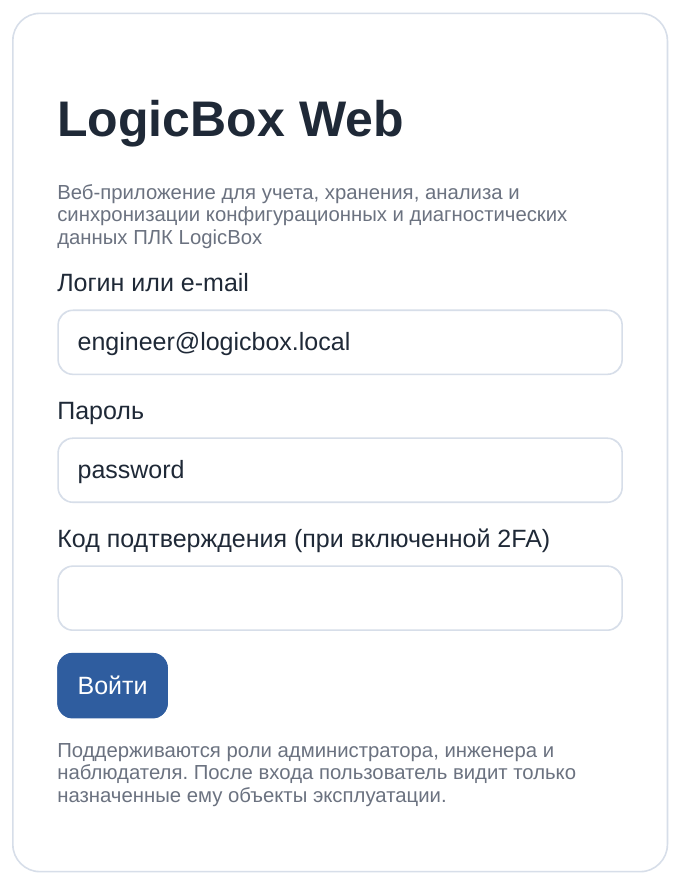
\includegraphics[width=0.90\textwidth,height=0.22\textheight,keepaspectratio]{images/mockups/login.png}
    \caption{Страница входа в систему}
\end{figure}
\vspace{2pt}

\begin{figure}[H]
    \centering
    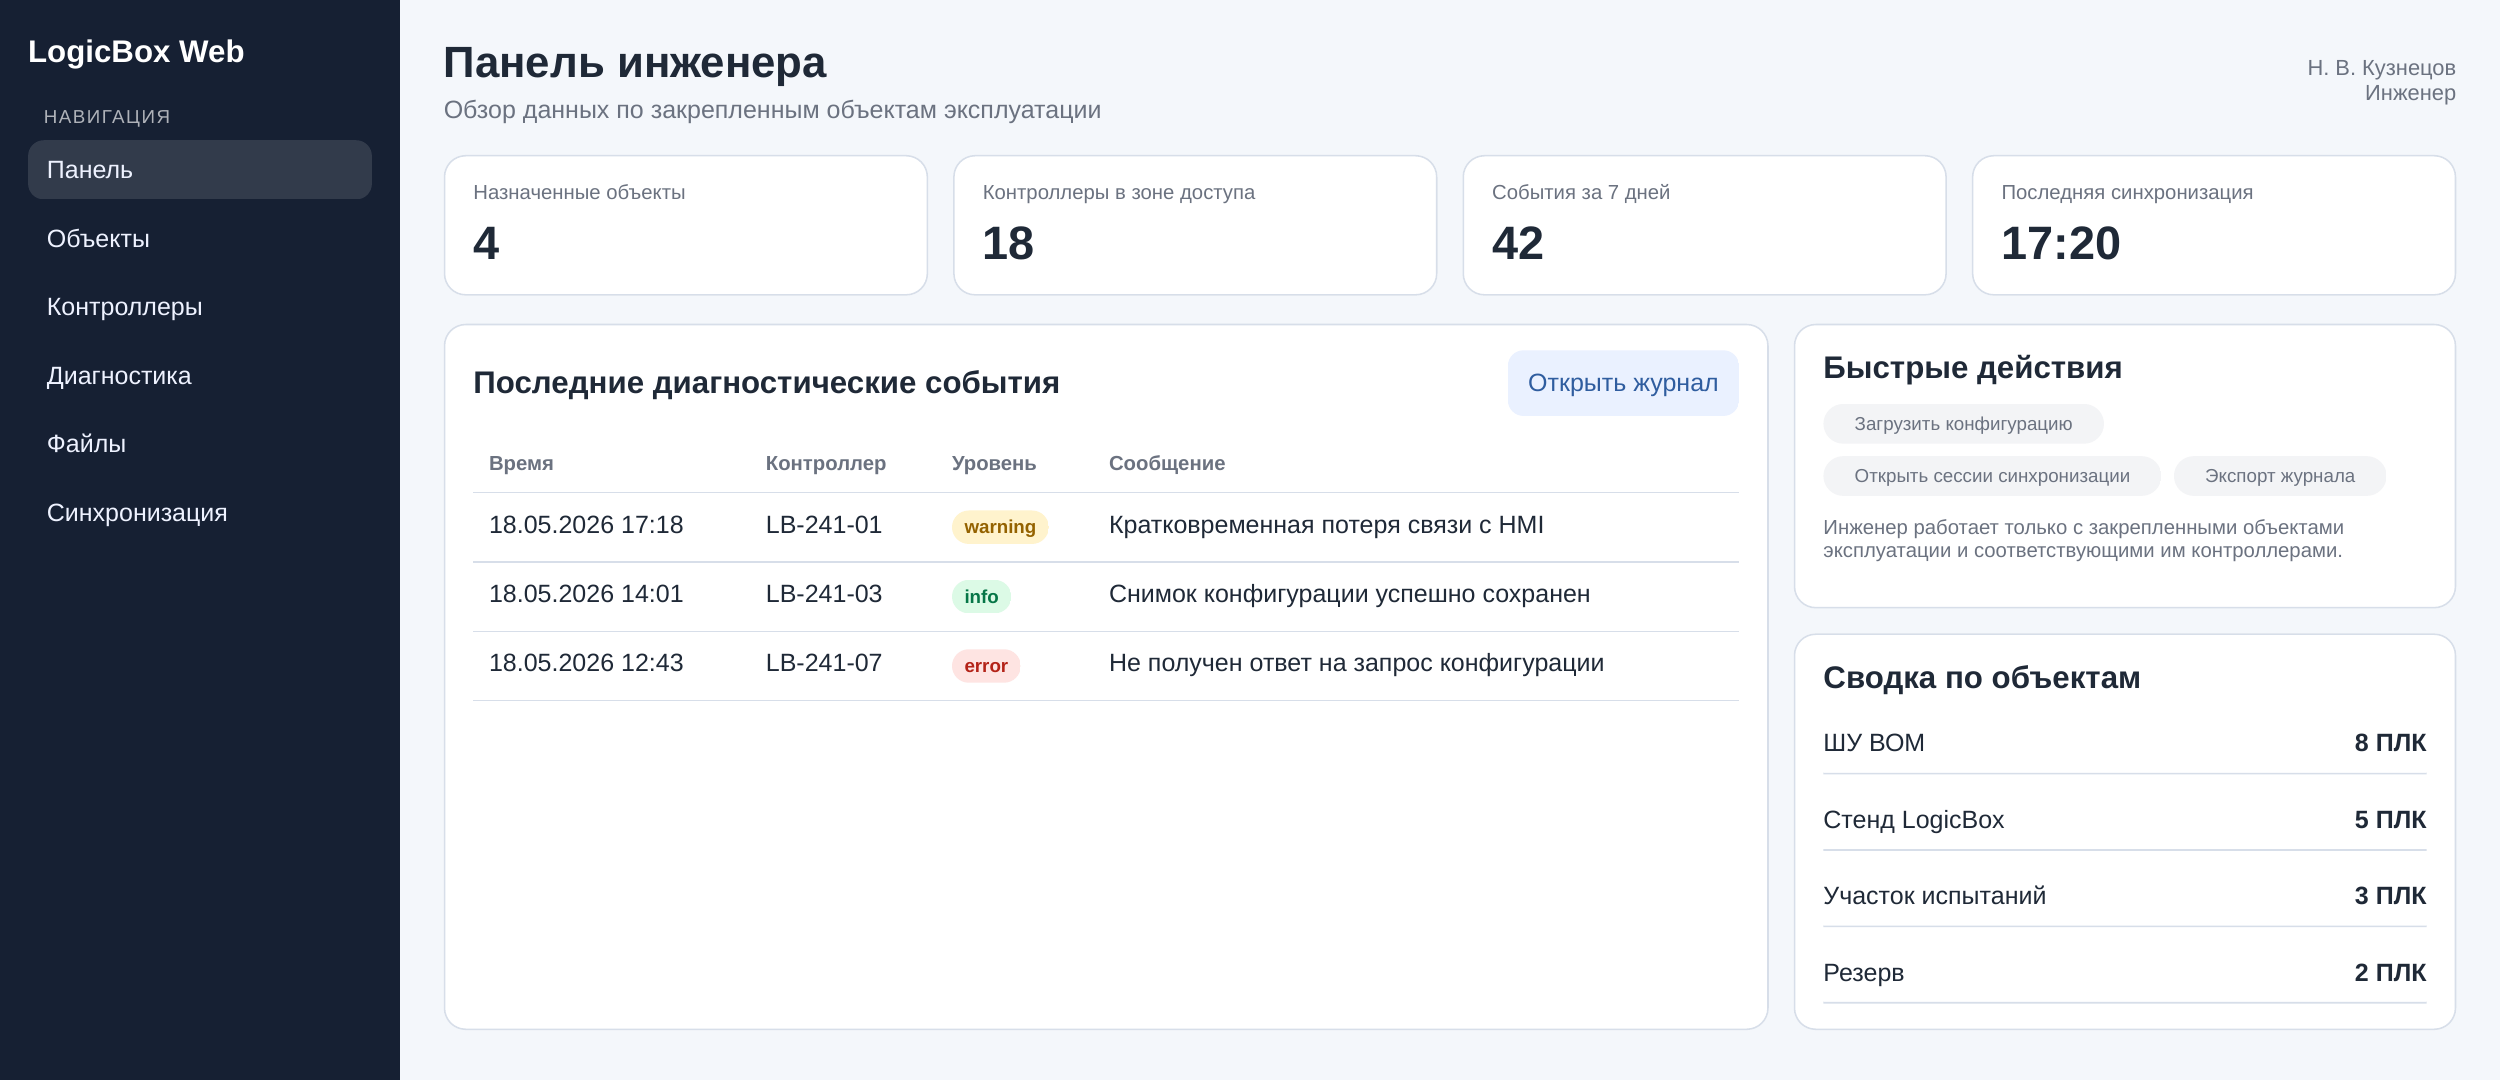
\includegraphics[width=0.90\textwidth,height=0.22\textheight,keepaspectratio]{images/mockups/dashboard_engineer.png}
    \caption{Панель инженера}
\end{figure}
\vspace{2pt}

\begin{figure}[H]
    \centering
    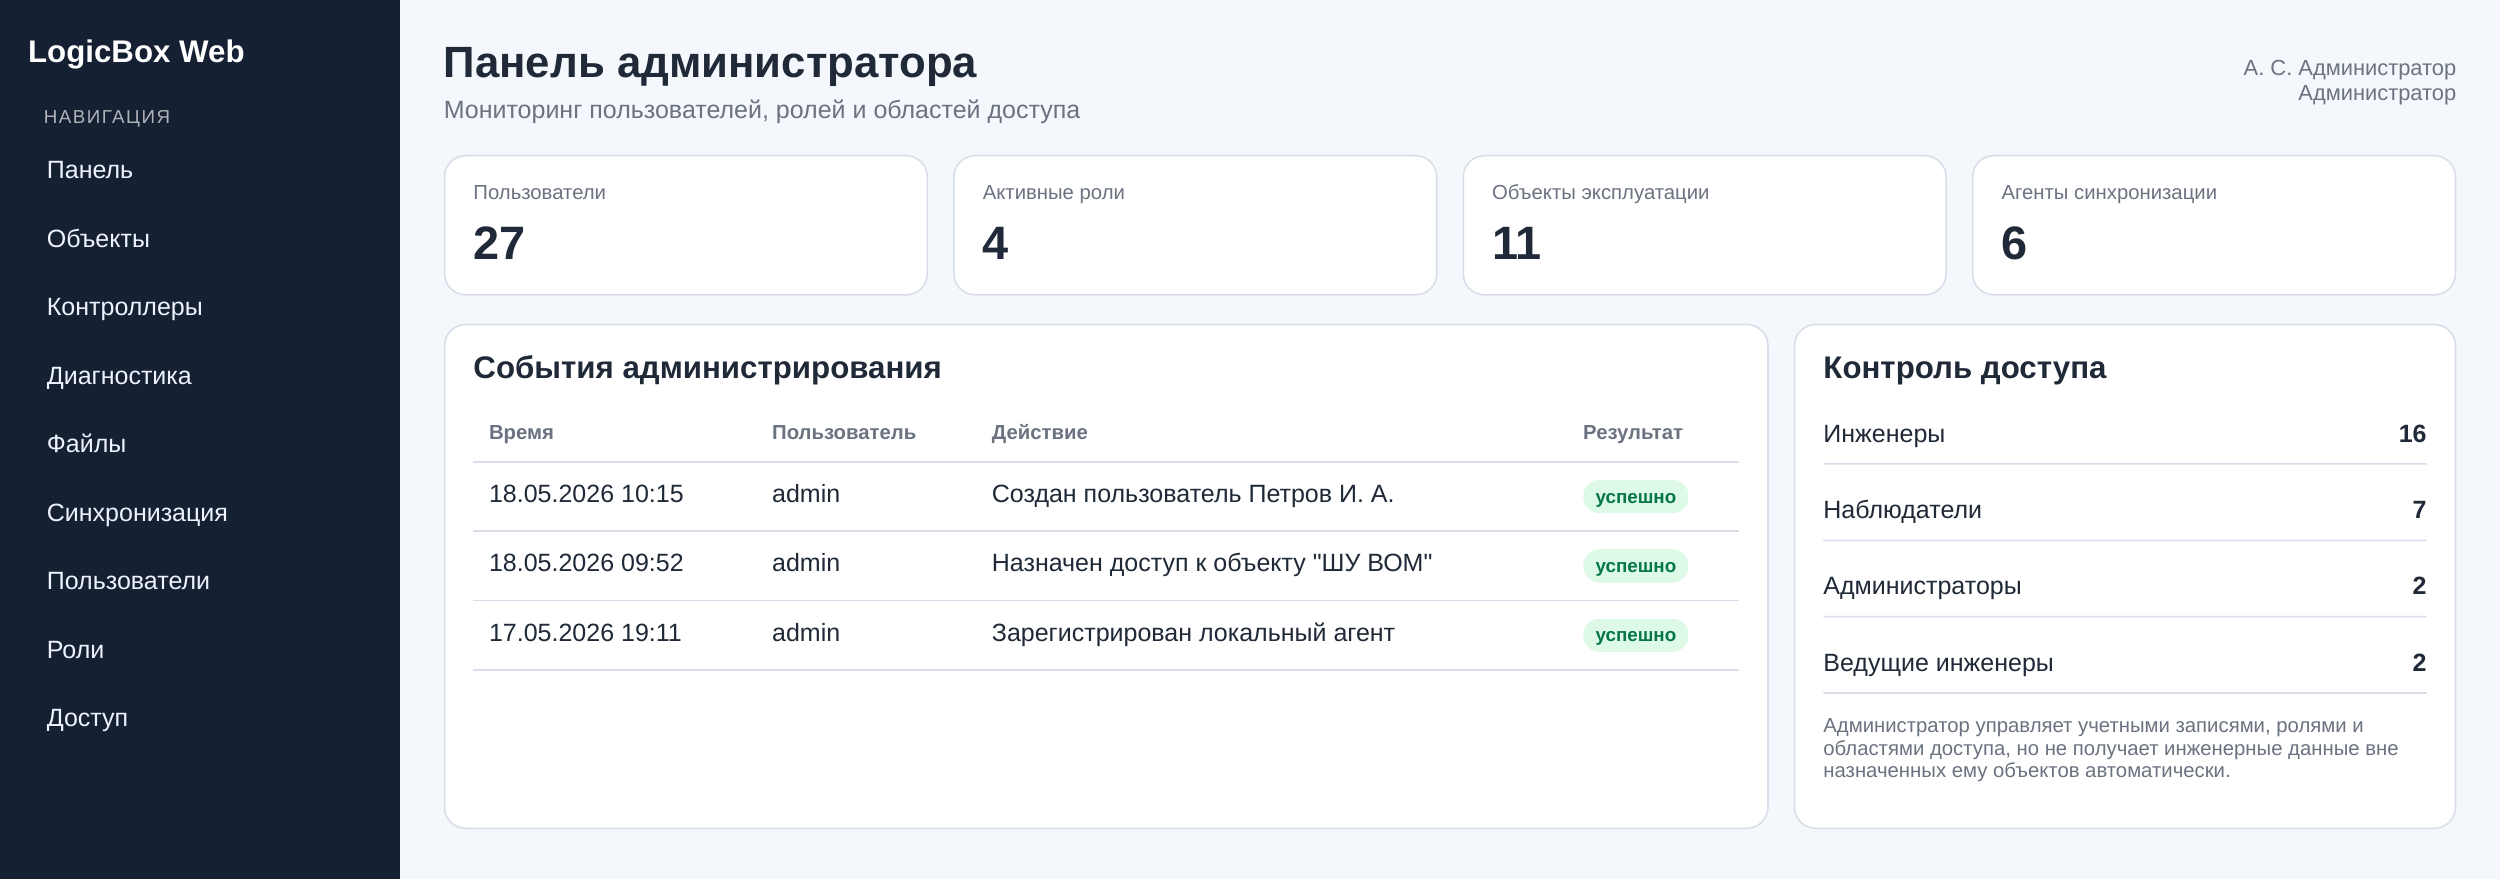
\includegraphics[width=0.90\textwidth,height=0.22\textheight,keepaspectratio]{images/mockups/dashboard_admin.png}
    \caption{Панель администратора}
\end{figure}
\vspace{2pt}

\begin{figure}[H]
    \centering
    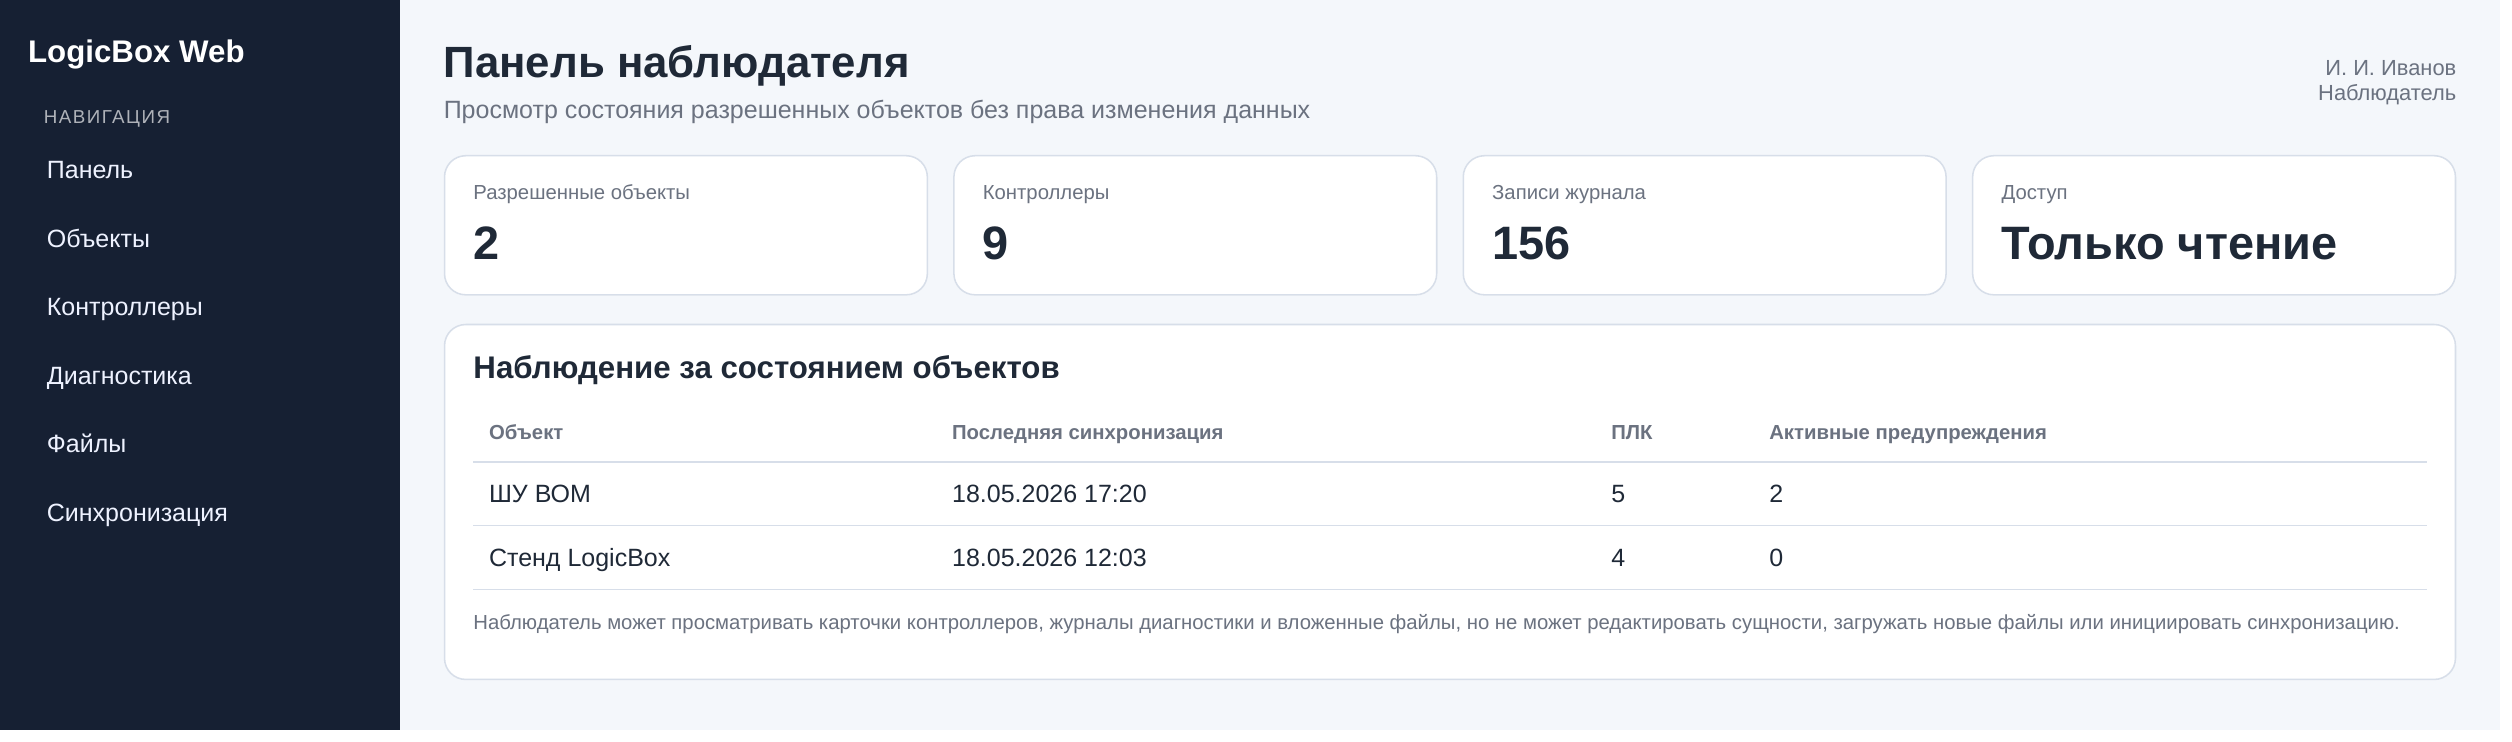
\includegraphics[width=0.90\textwidth,height=0.22\textheight,keepaspectratio]{images/mockups/dashboard_observer.png}
    \caption{Панель наблюдателя}
\end{figure}
\vspace{2pt}

\begin{figure}[H]
    \centering
    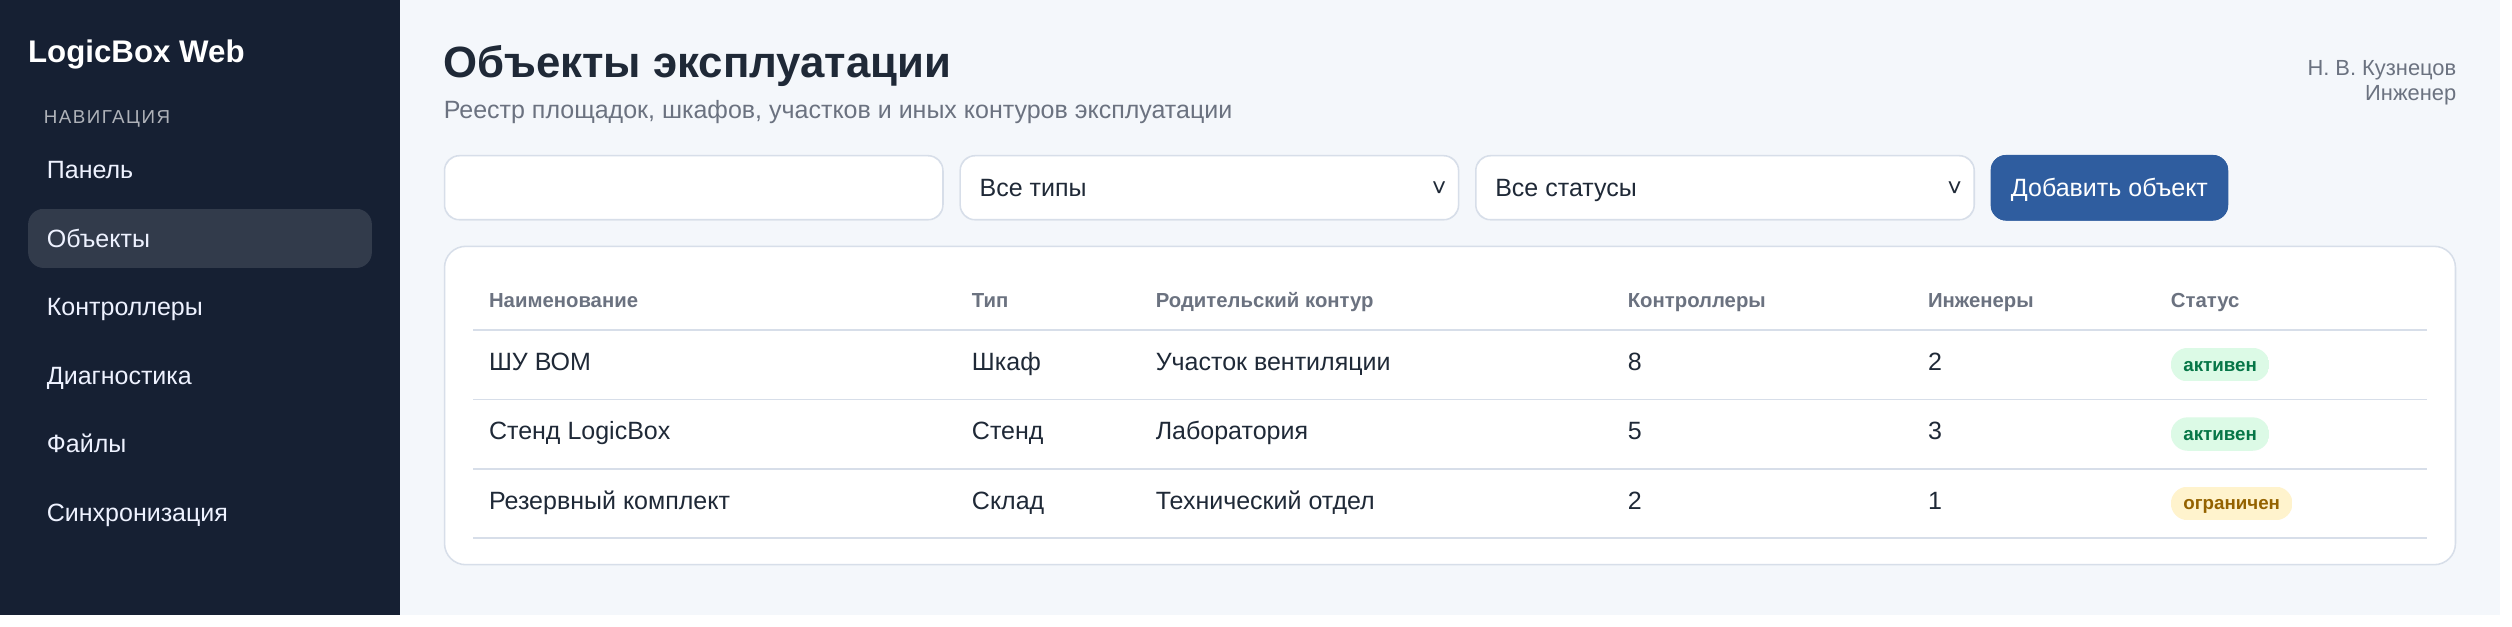
\includegraphics[width=0.90\textwidth,height=0.22\textheight,keepaspectratio]{images/mockups/objects.png}
    \caption{Реестр объектов эксплуатации}
\end{figure}
\vspace{2pt}

\begin{figure}[H]
    \centering
    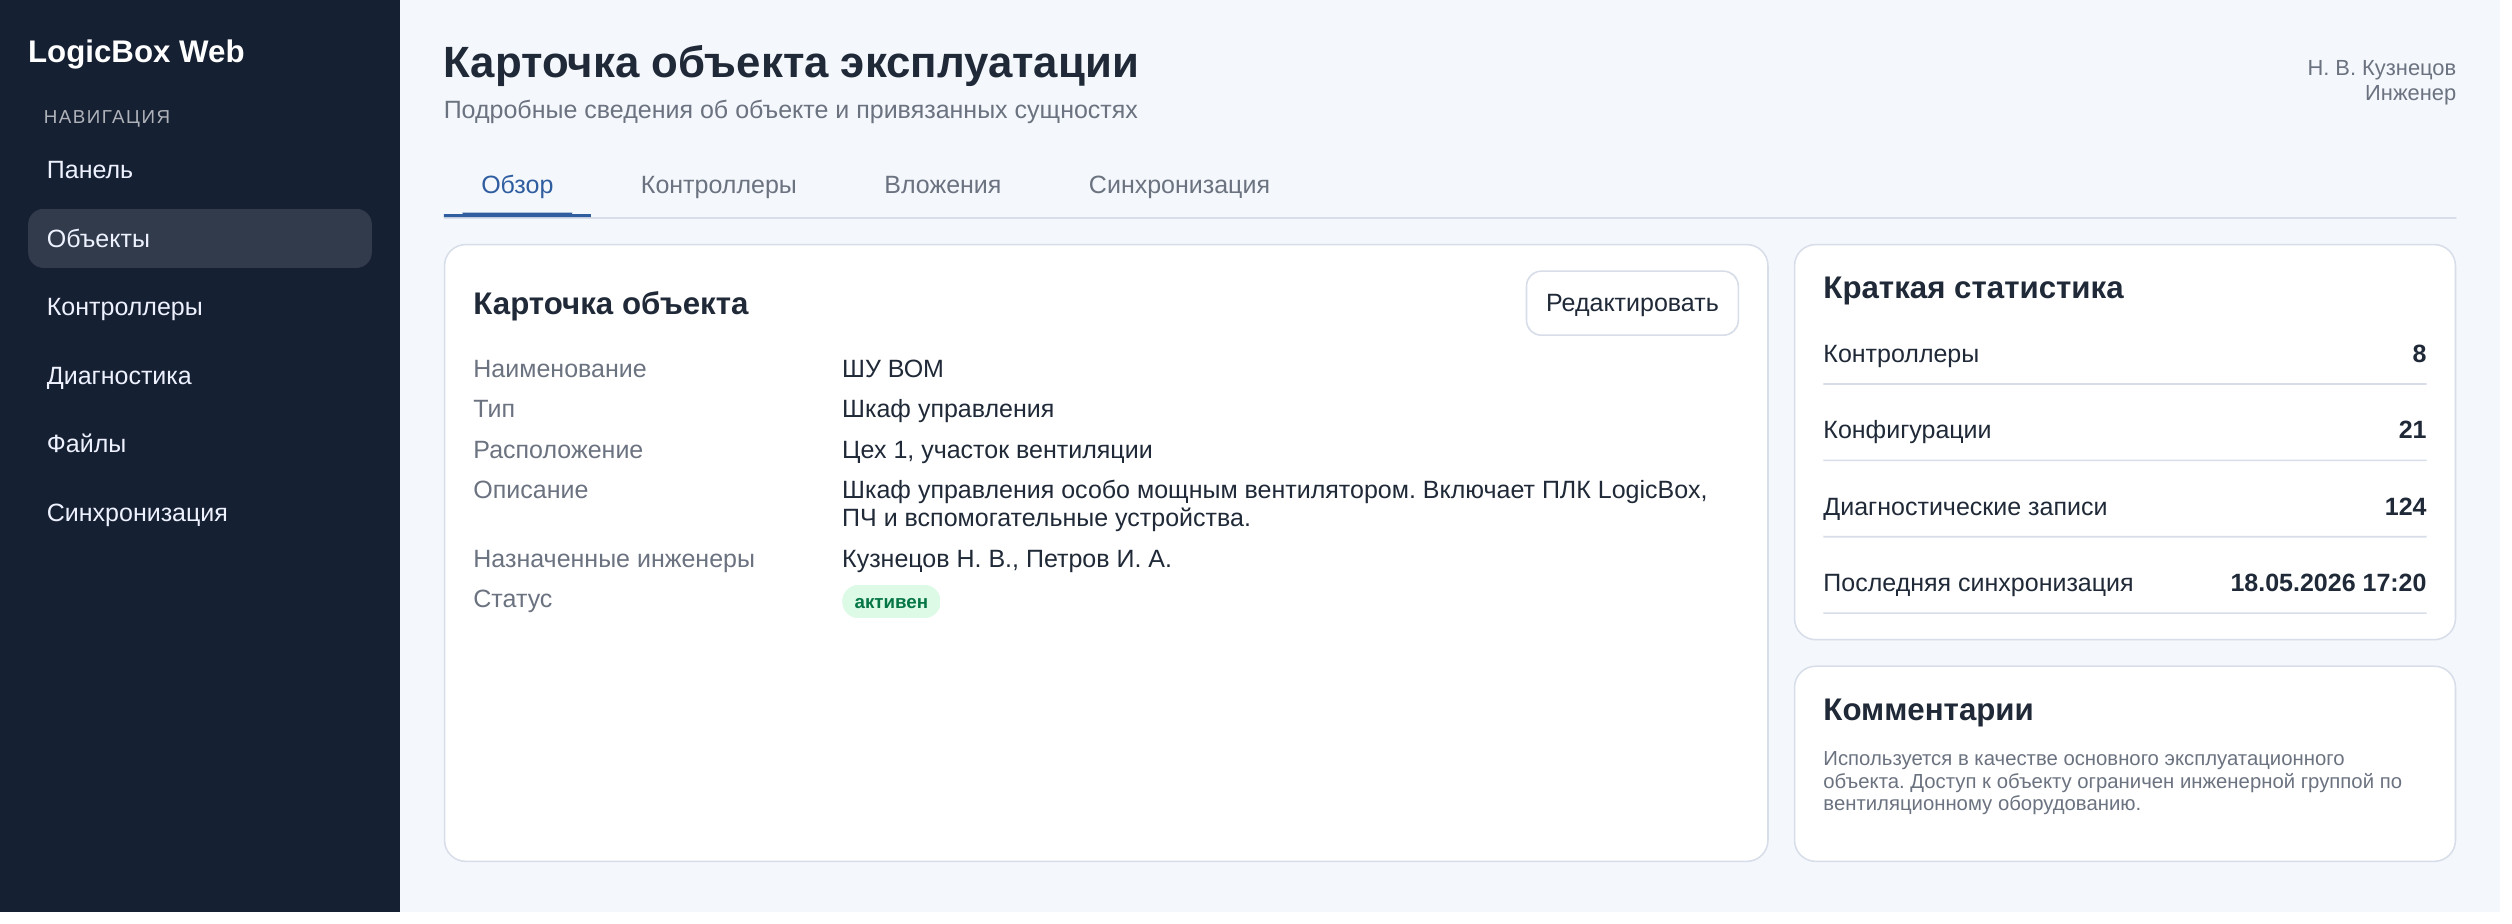
\includegraphics[width=0.90\textwidth,height=0.22\textheight,keepaspectratio]{images/mockups/object_card.png}
    \caption{Карточка объекта эксплуатации}
\end{figure}
\vspace{2pt}

\begin{figure}[H]
    \centering
    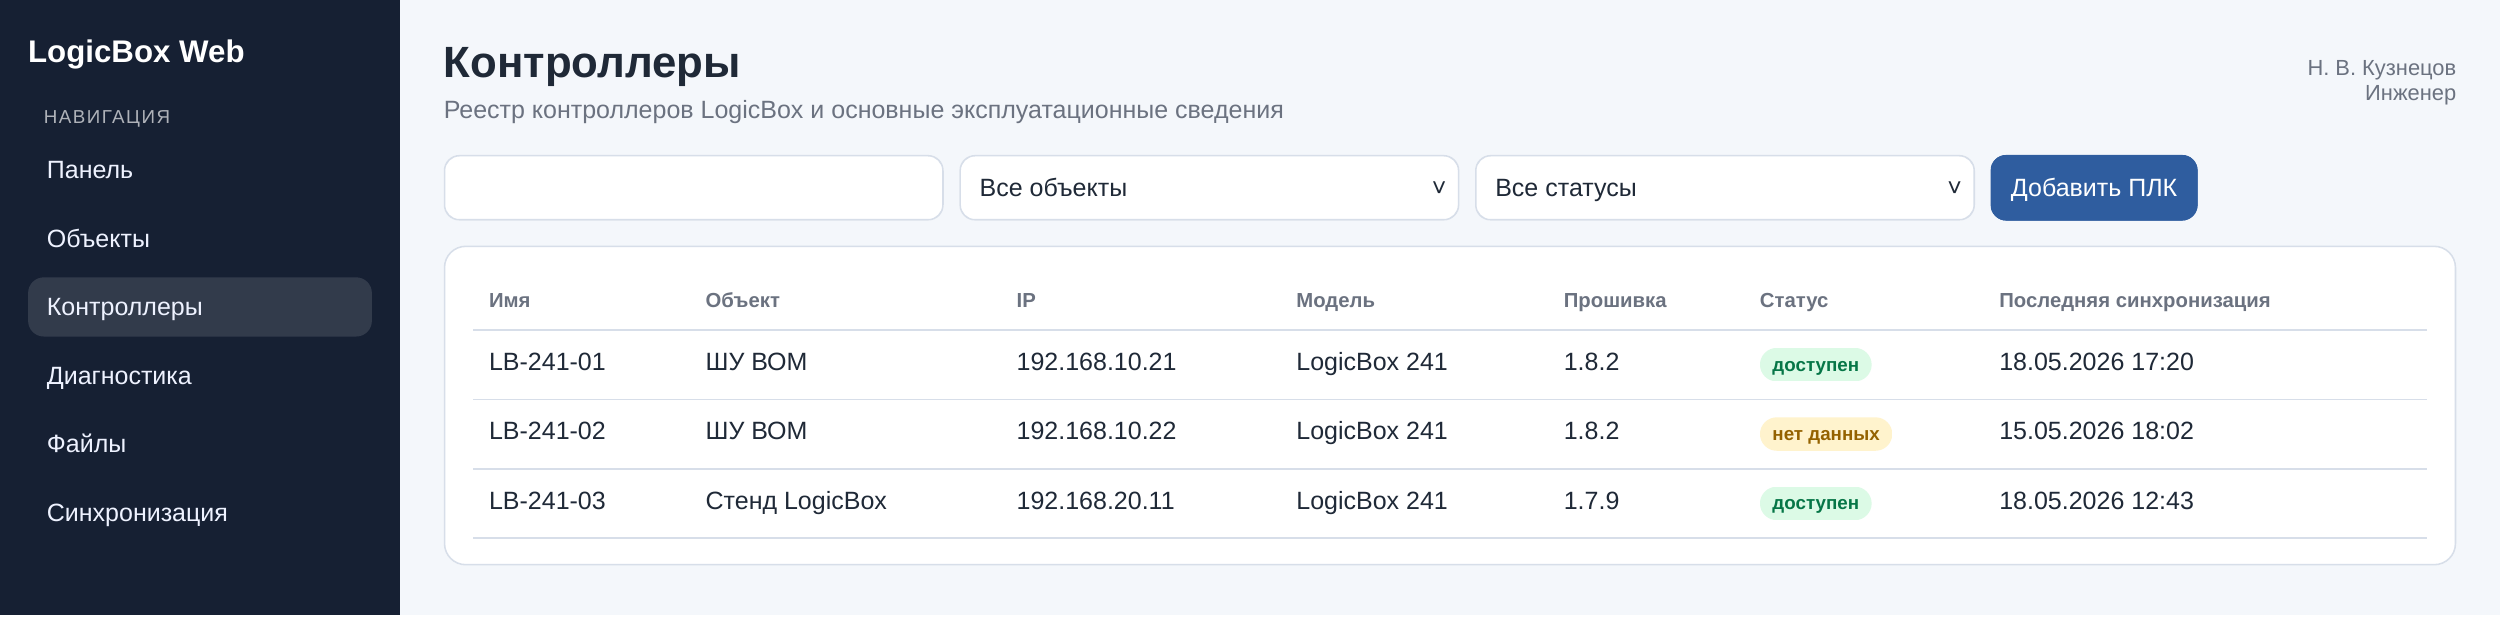
\includegraphics[width=0.90\textwidth,height=0.22\textheight,keepaspectratio]{images/mockups/controllers.png}
    \caption{Список контроллеров}
\end{figure}
\vspace{2pt}

\begin{figure}[H]
    \centering
    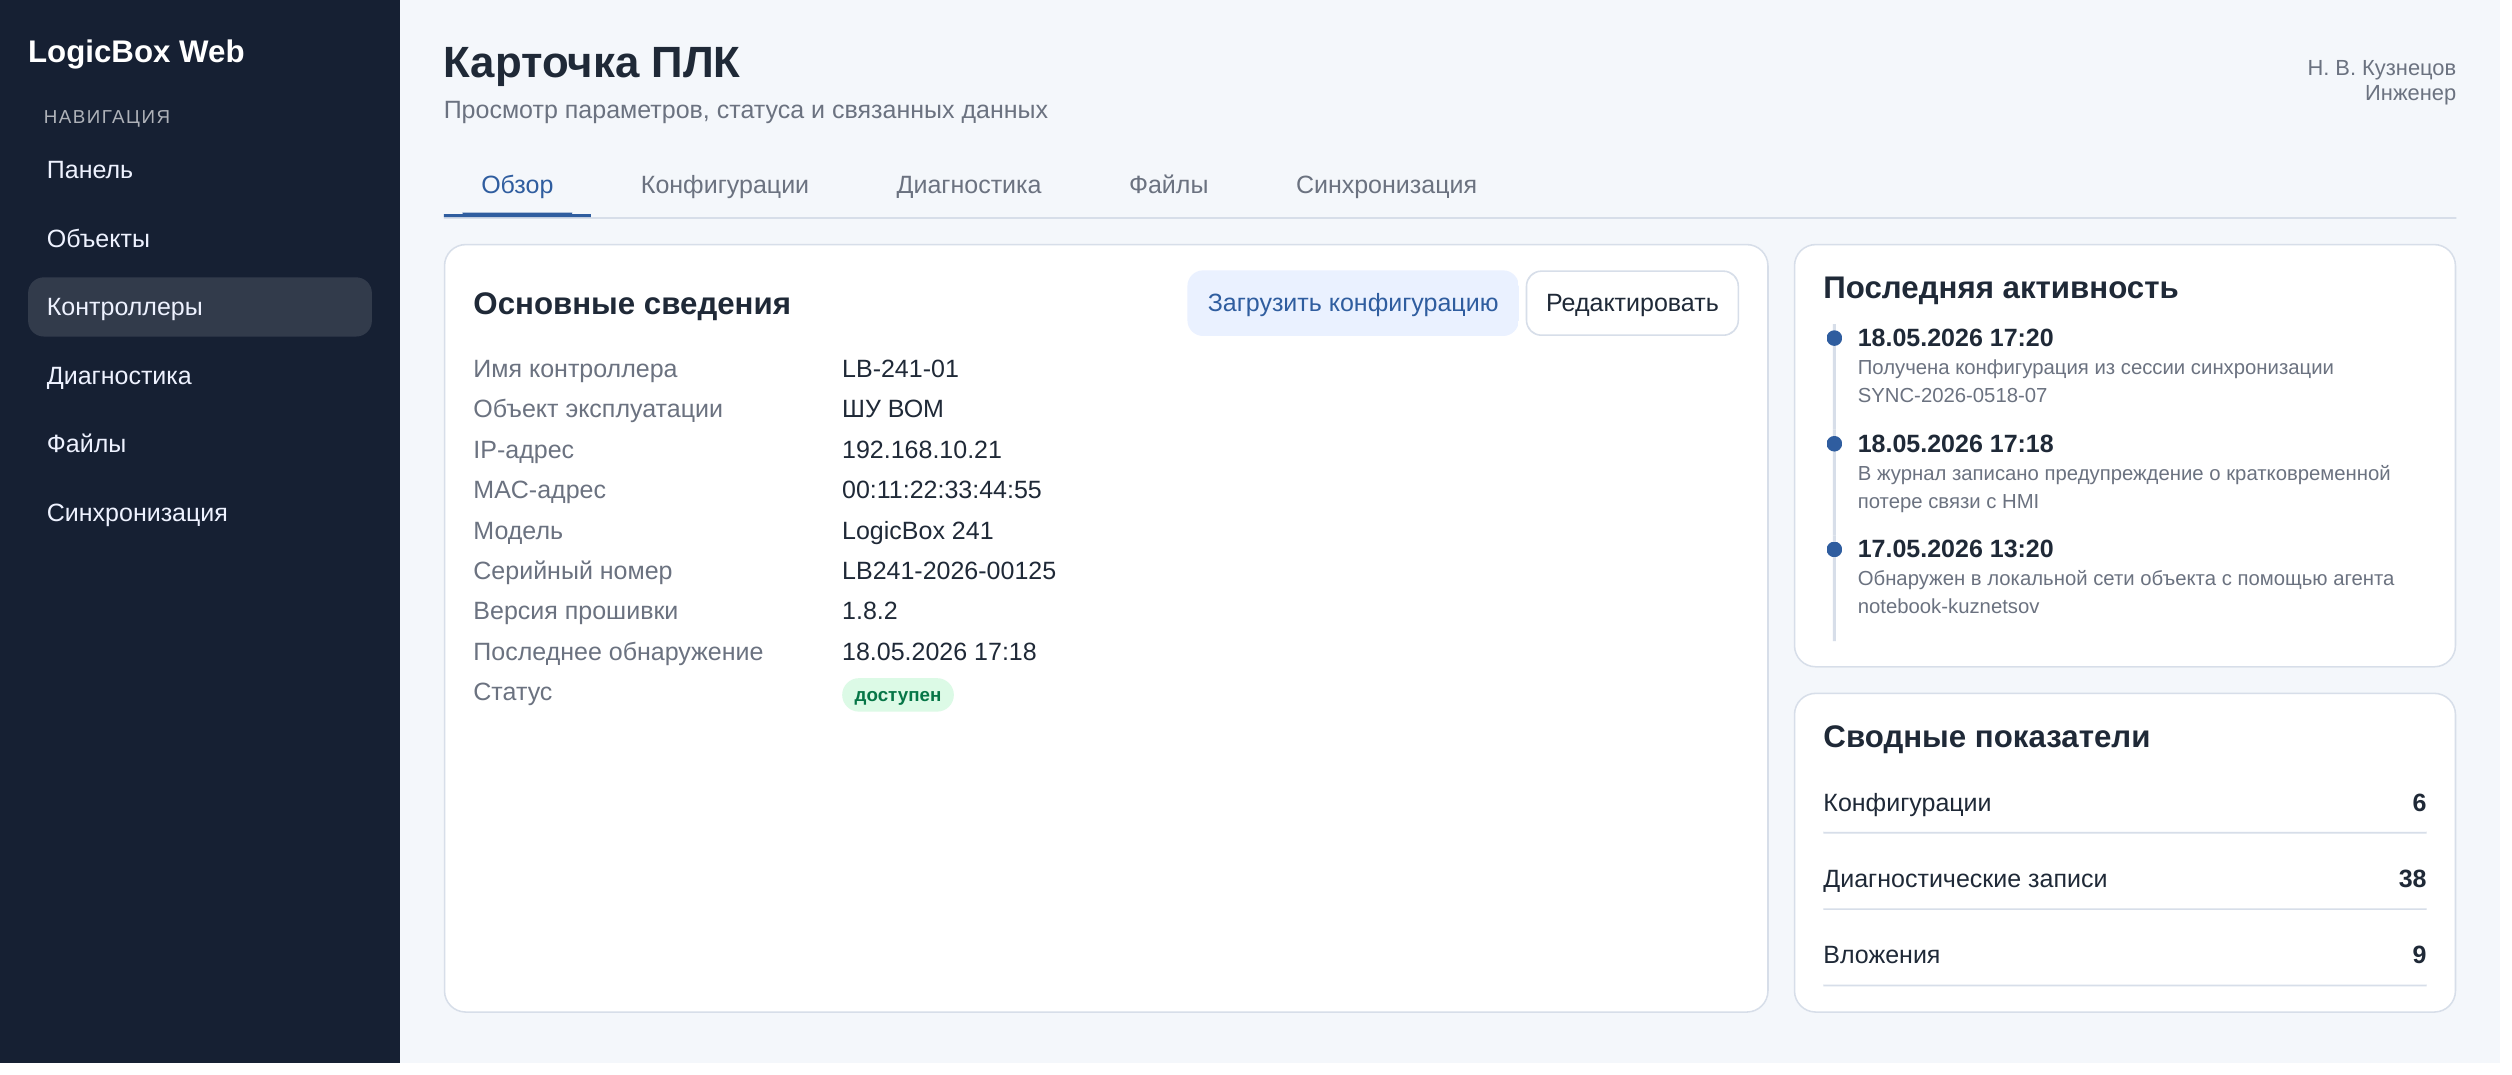
\includegraphics[width=0.90\textwidth,height=0.22\textheight,keepaspectratio]{images/mockups/controller_card_overview.png}
    \caption{Карточка контроллера: обзор}
\end{figure}
\vspace{2pt}

\begin{figure}[H]
    \centering
    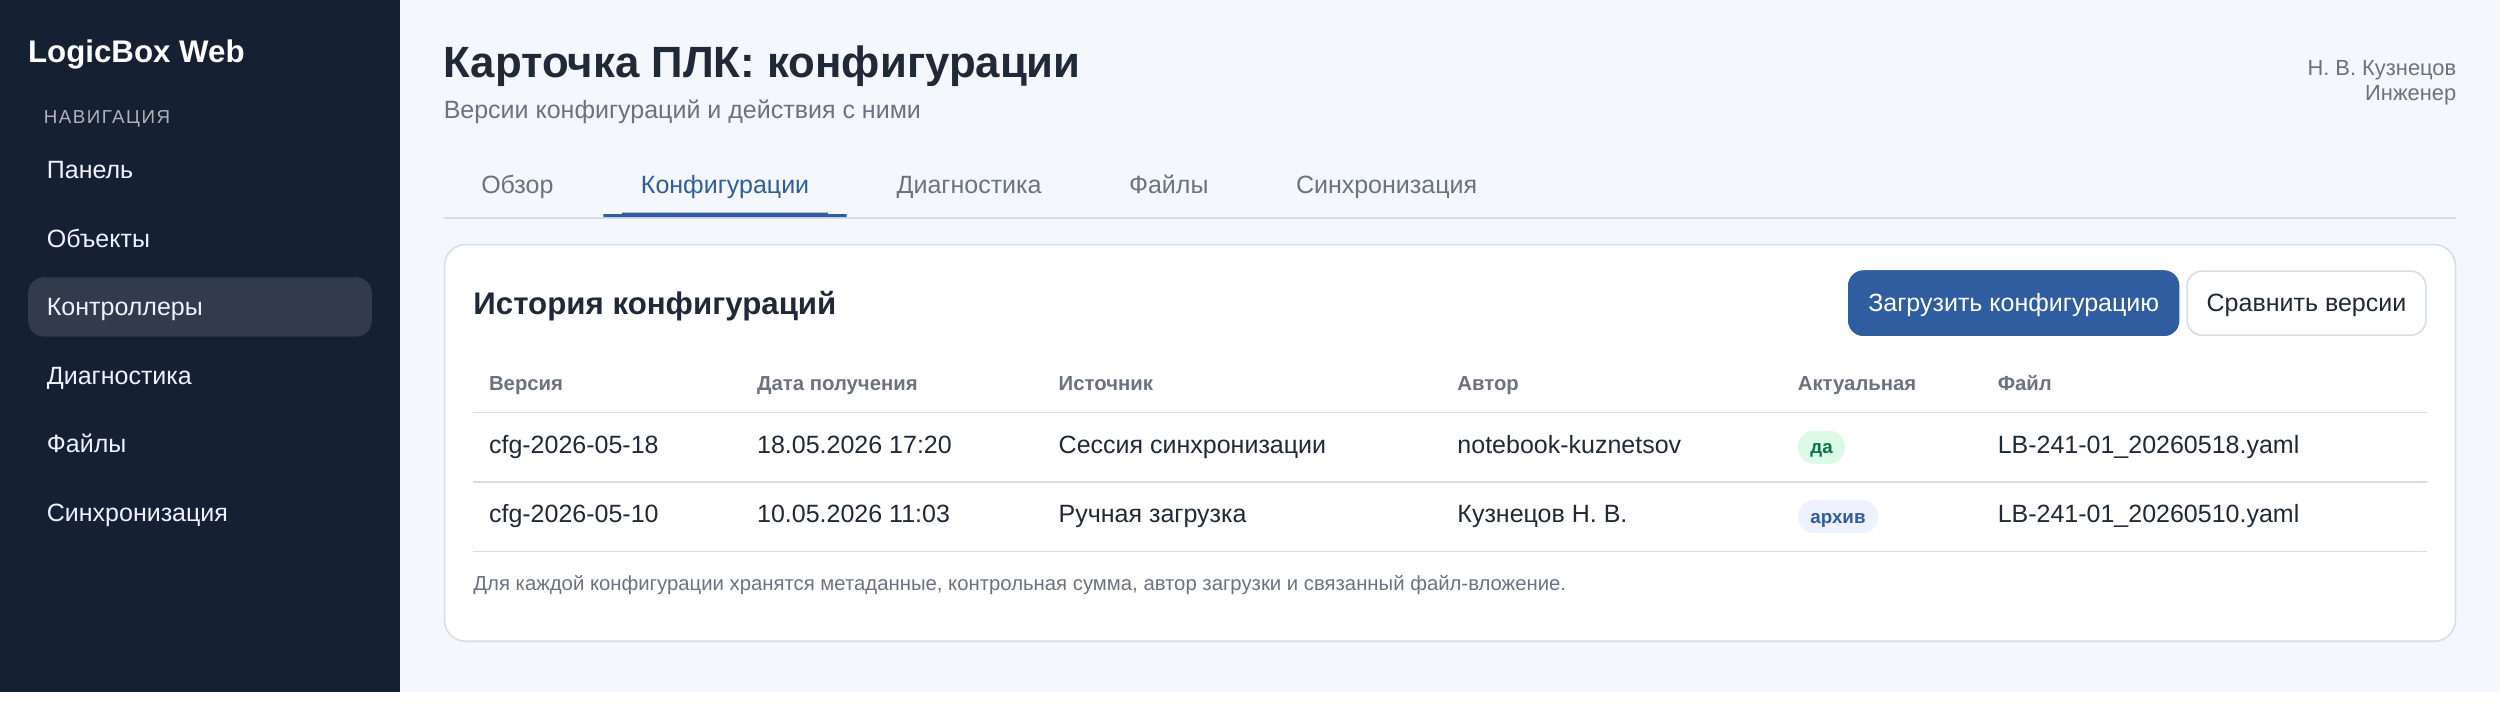
\includegraphics[width=0.90\textwidth,height=0.22\textheight,keepaspectratio]{images/mockups/controller_card_configs.png}
    \caption{Карточка контроллера: конфигурации}
\end{figure}
\vspace{2pt}

\begin{figure}[H]
    \centering
    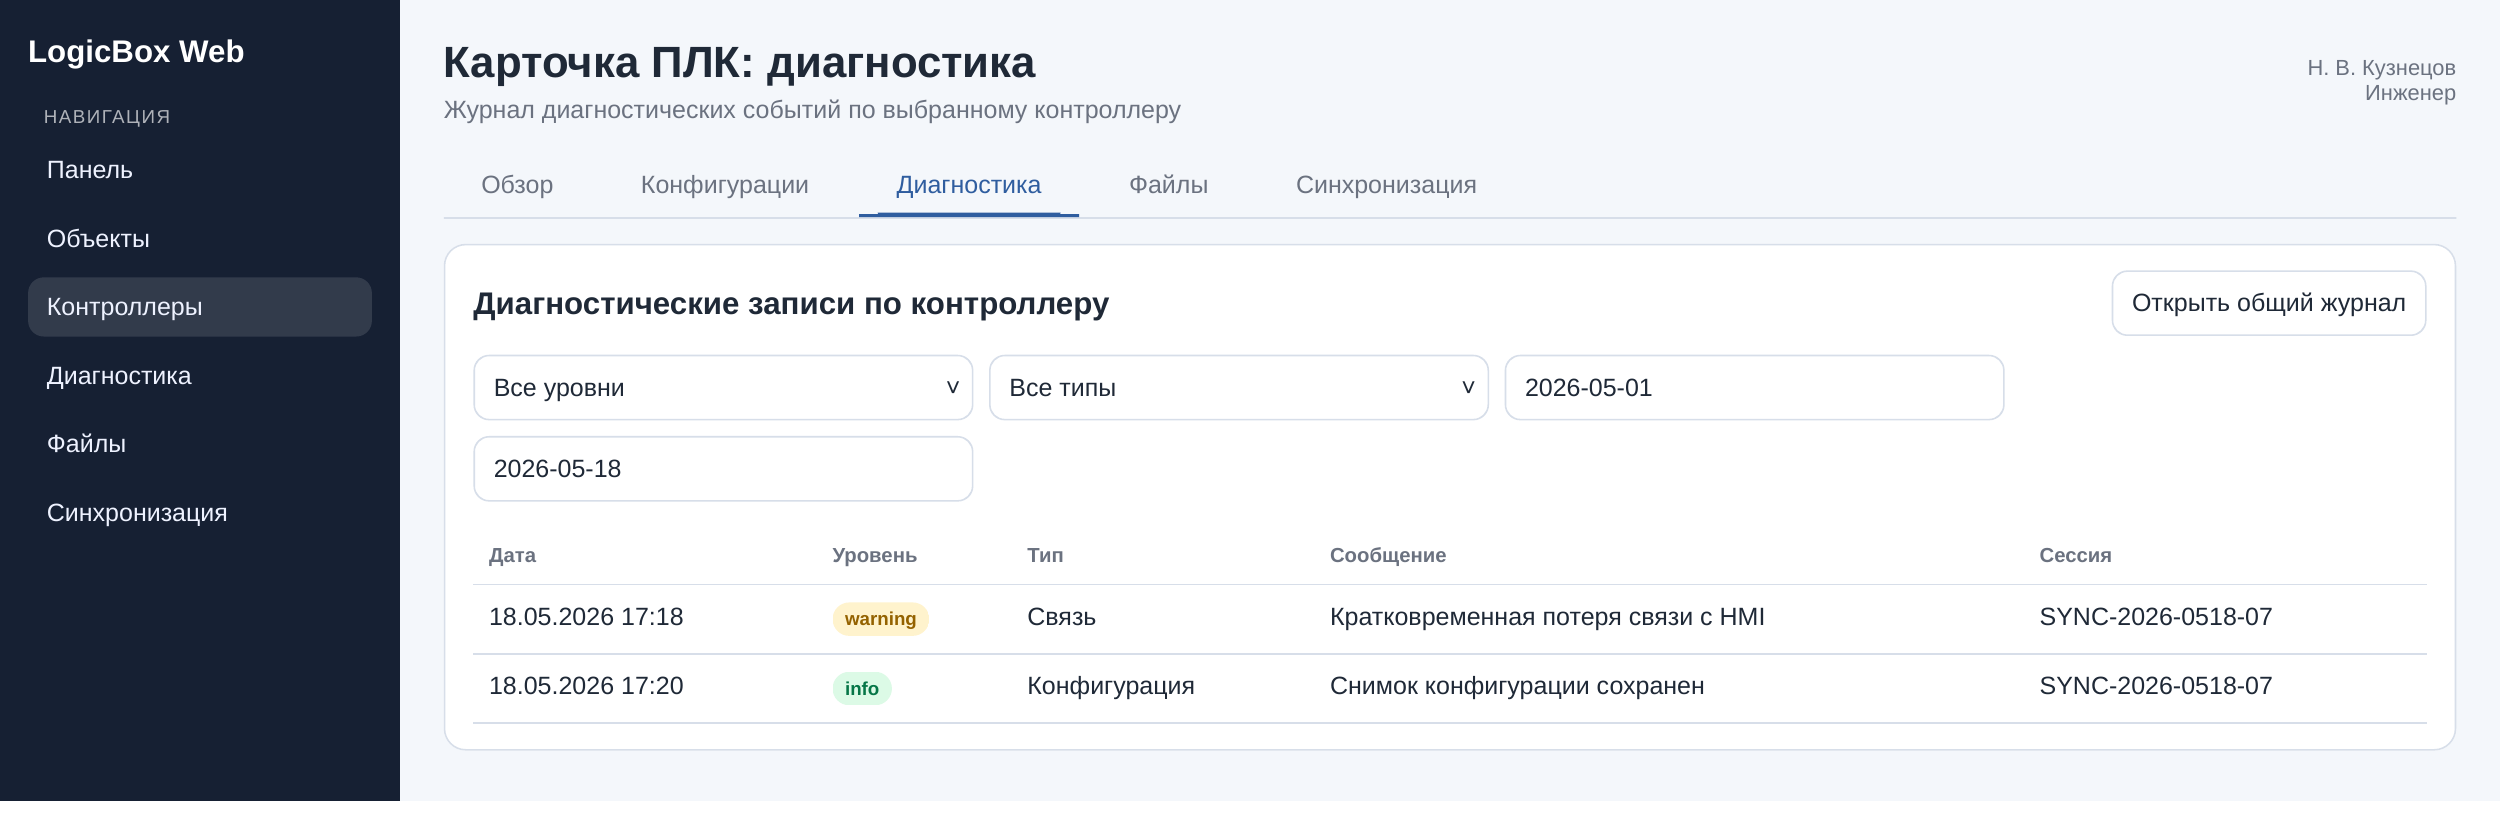
\includegraphics[width=0.90\textwidth,height=0.22\textheight,keepaspectratio]{images/mockups/controller_card_diagnostics.png}
    \caption{Карточка контроллера: диагностика}
\end{figure}
\vspace{2pt}

\begin{figure}[H]
    \centering
    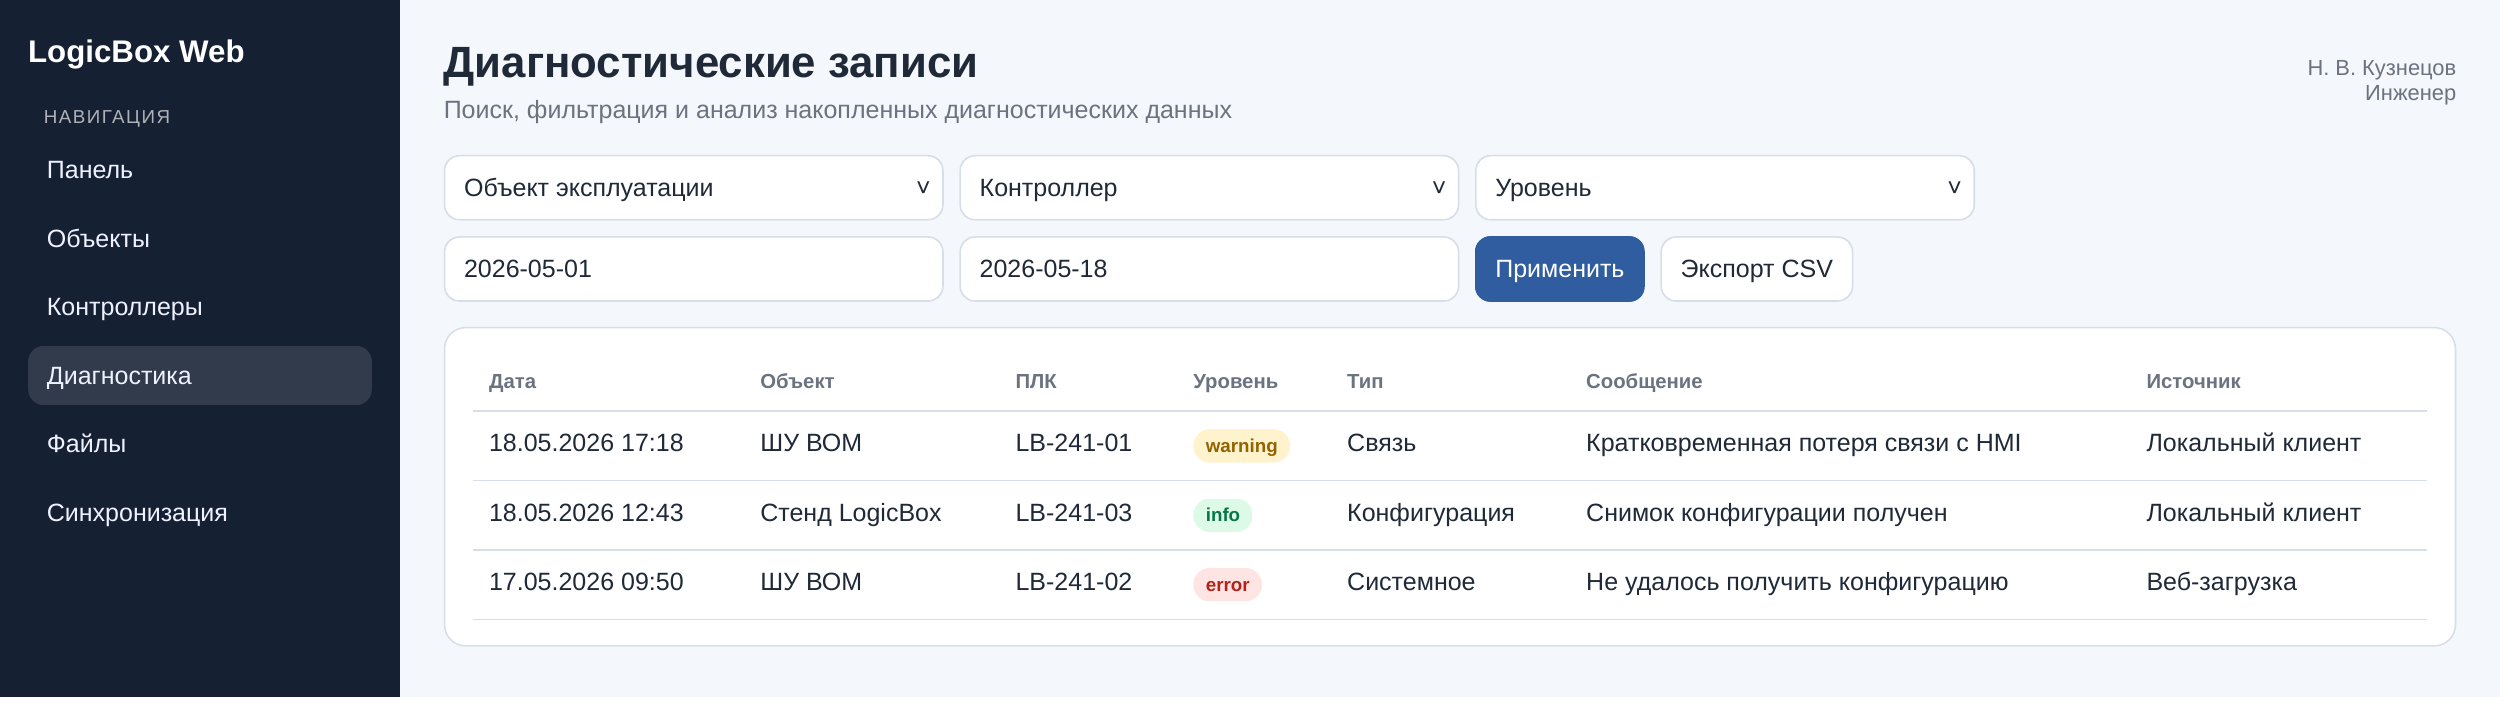
\includegraphics[width=0.90\textwidth,height=0.22\textheight,keepaspectratio]{images/mockups/diagnostics.png}
    \caption{Общий журнал диагностических записей}
\end{figure}
\vspace{2pt}

\begin{figure}[H]
    \centering
    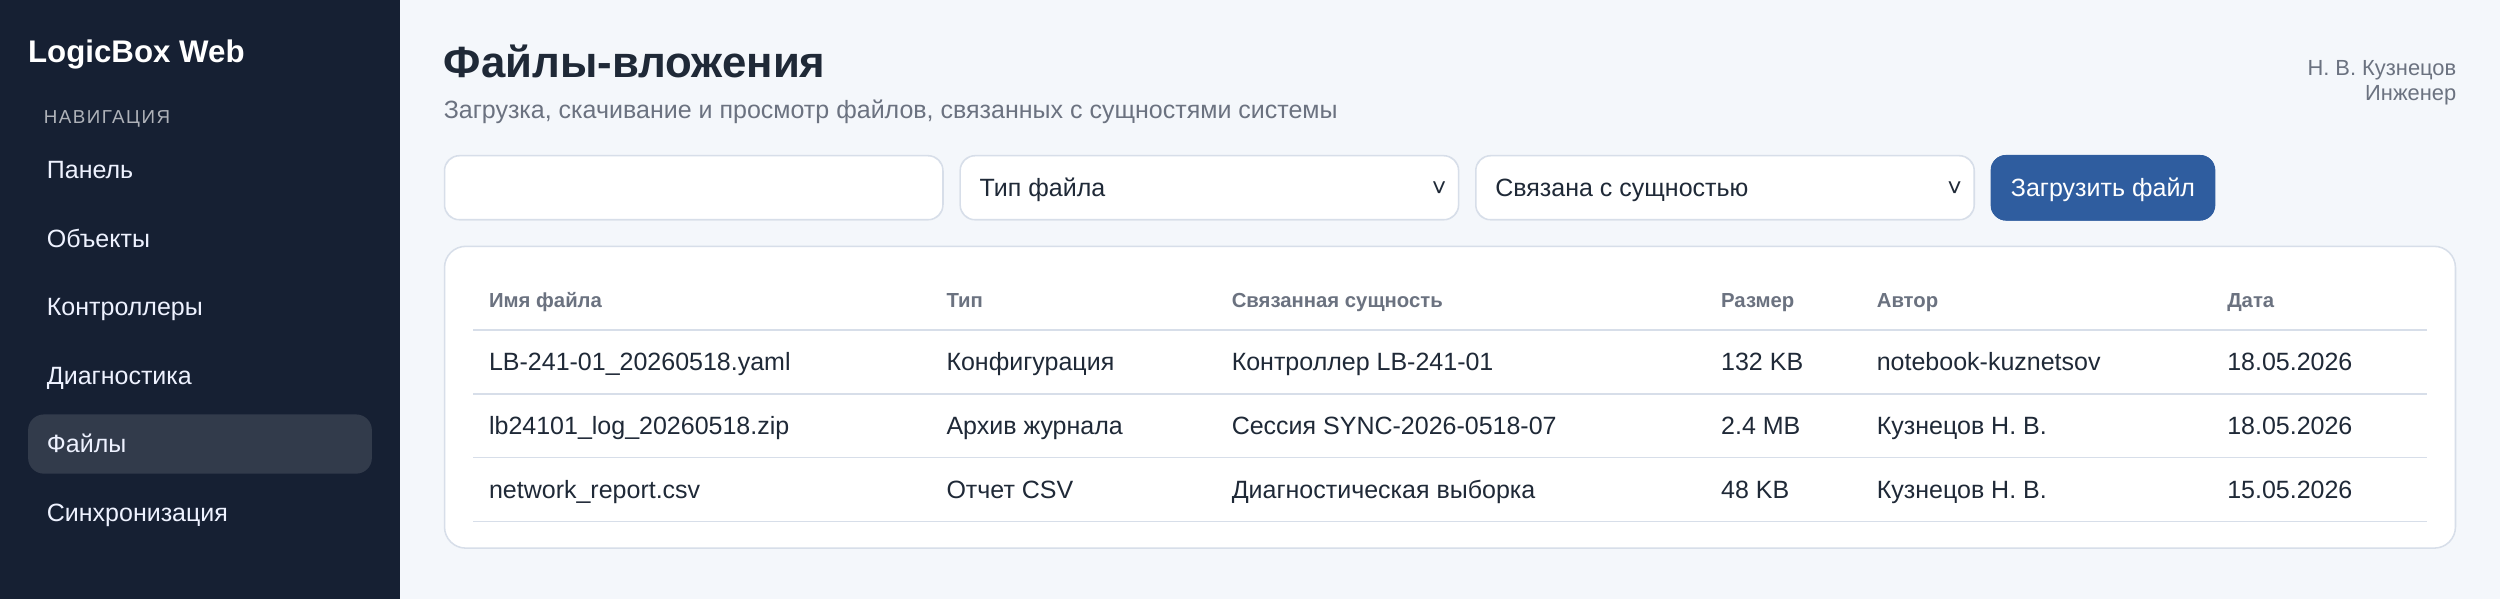
\includegraphics[width=0.90\textwidth,height=0.22\textheight,keepaspectratio]{images/mockups/attachments.png}
    \caption{Страница файлов-вложений}
\end{figure}
\vspace{2pt}

\begin{figure}[H]
    \centering
    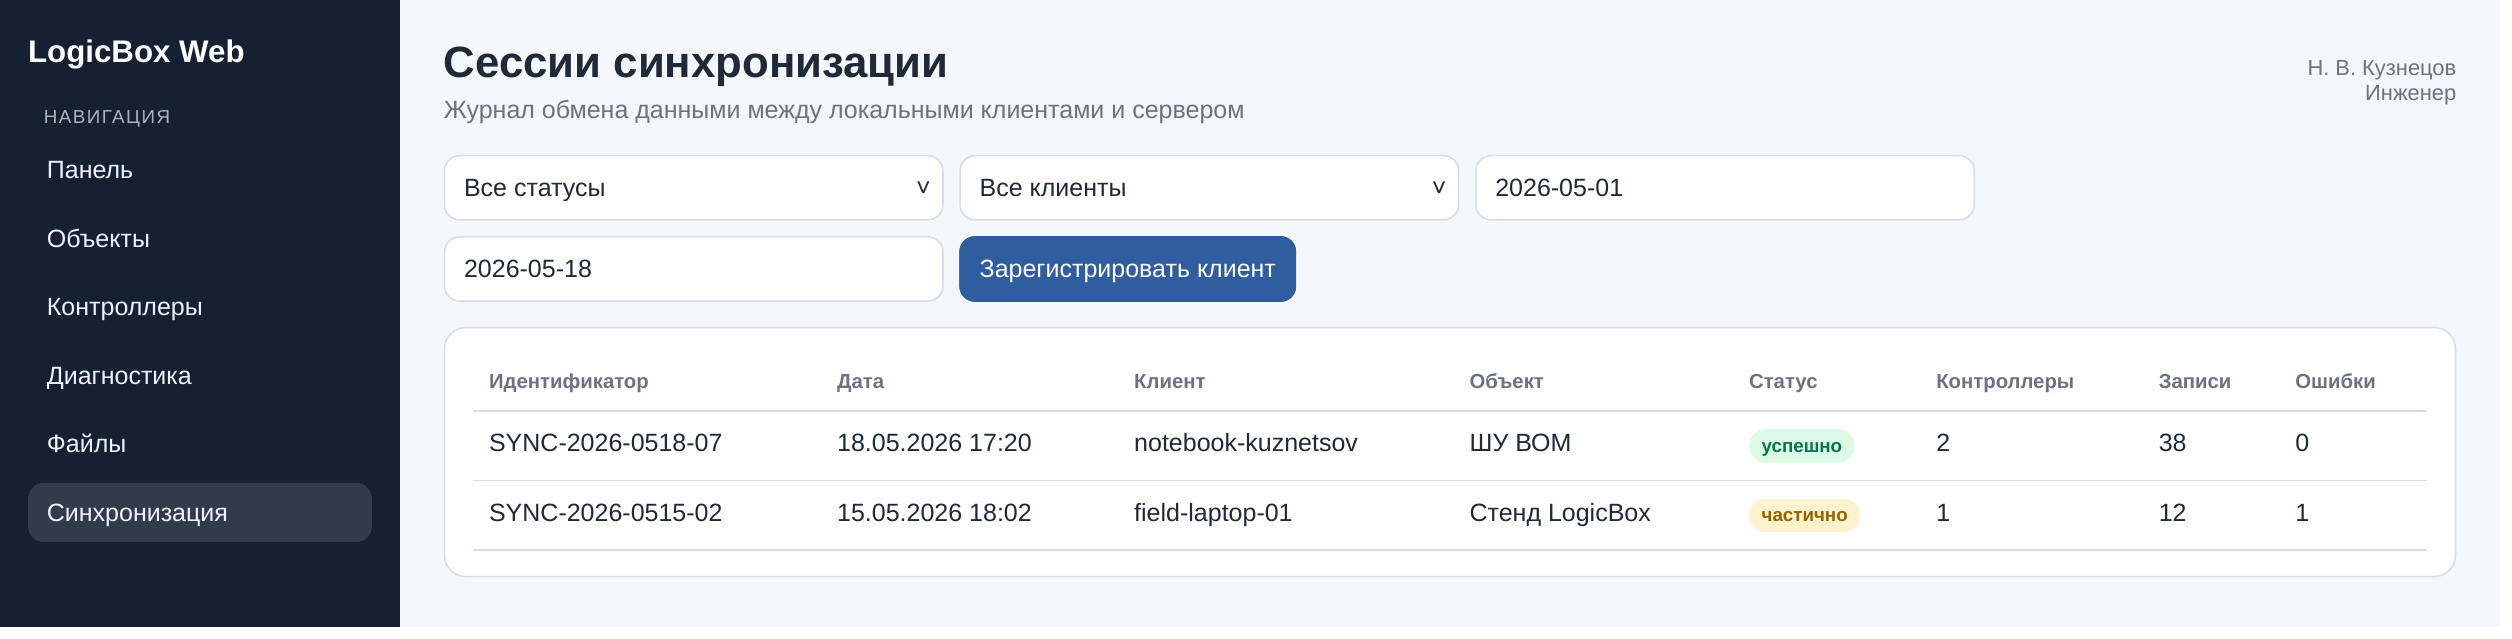
\includegraphics[width=0.90\textwidth,height=0.22\textheight,keepaspectratio]{images/mockups/sync_sessions.png}
    \caption{Журнал сессий синхронизации}
\end{figure}
\vspace{2pt}

\begin{figure}[H]
    \centering
    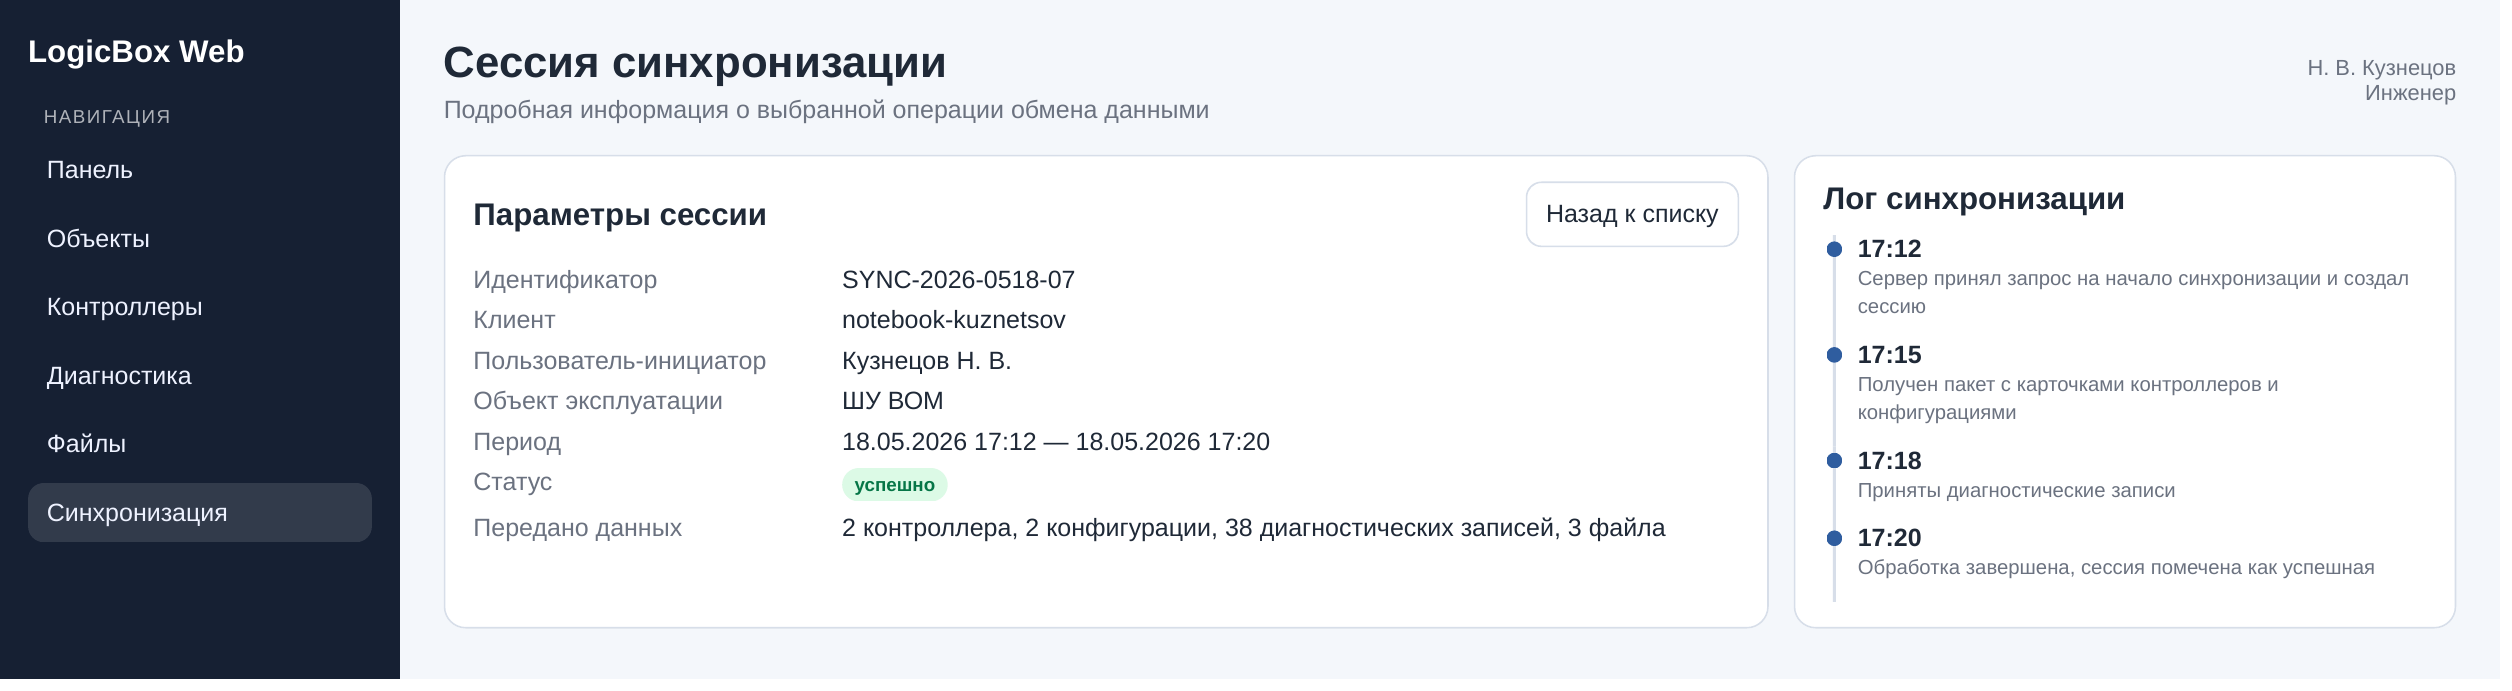
\includegraphics[width=0.90\textwidth,height=0.22\textheight,keepaspectratio]{images/mockups/sync_session_card.png}
    \caption{Карточка сессии синхронизации}
\end{figure}
\vspace{2pt}

\begin{figure}[H]
    \centering
    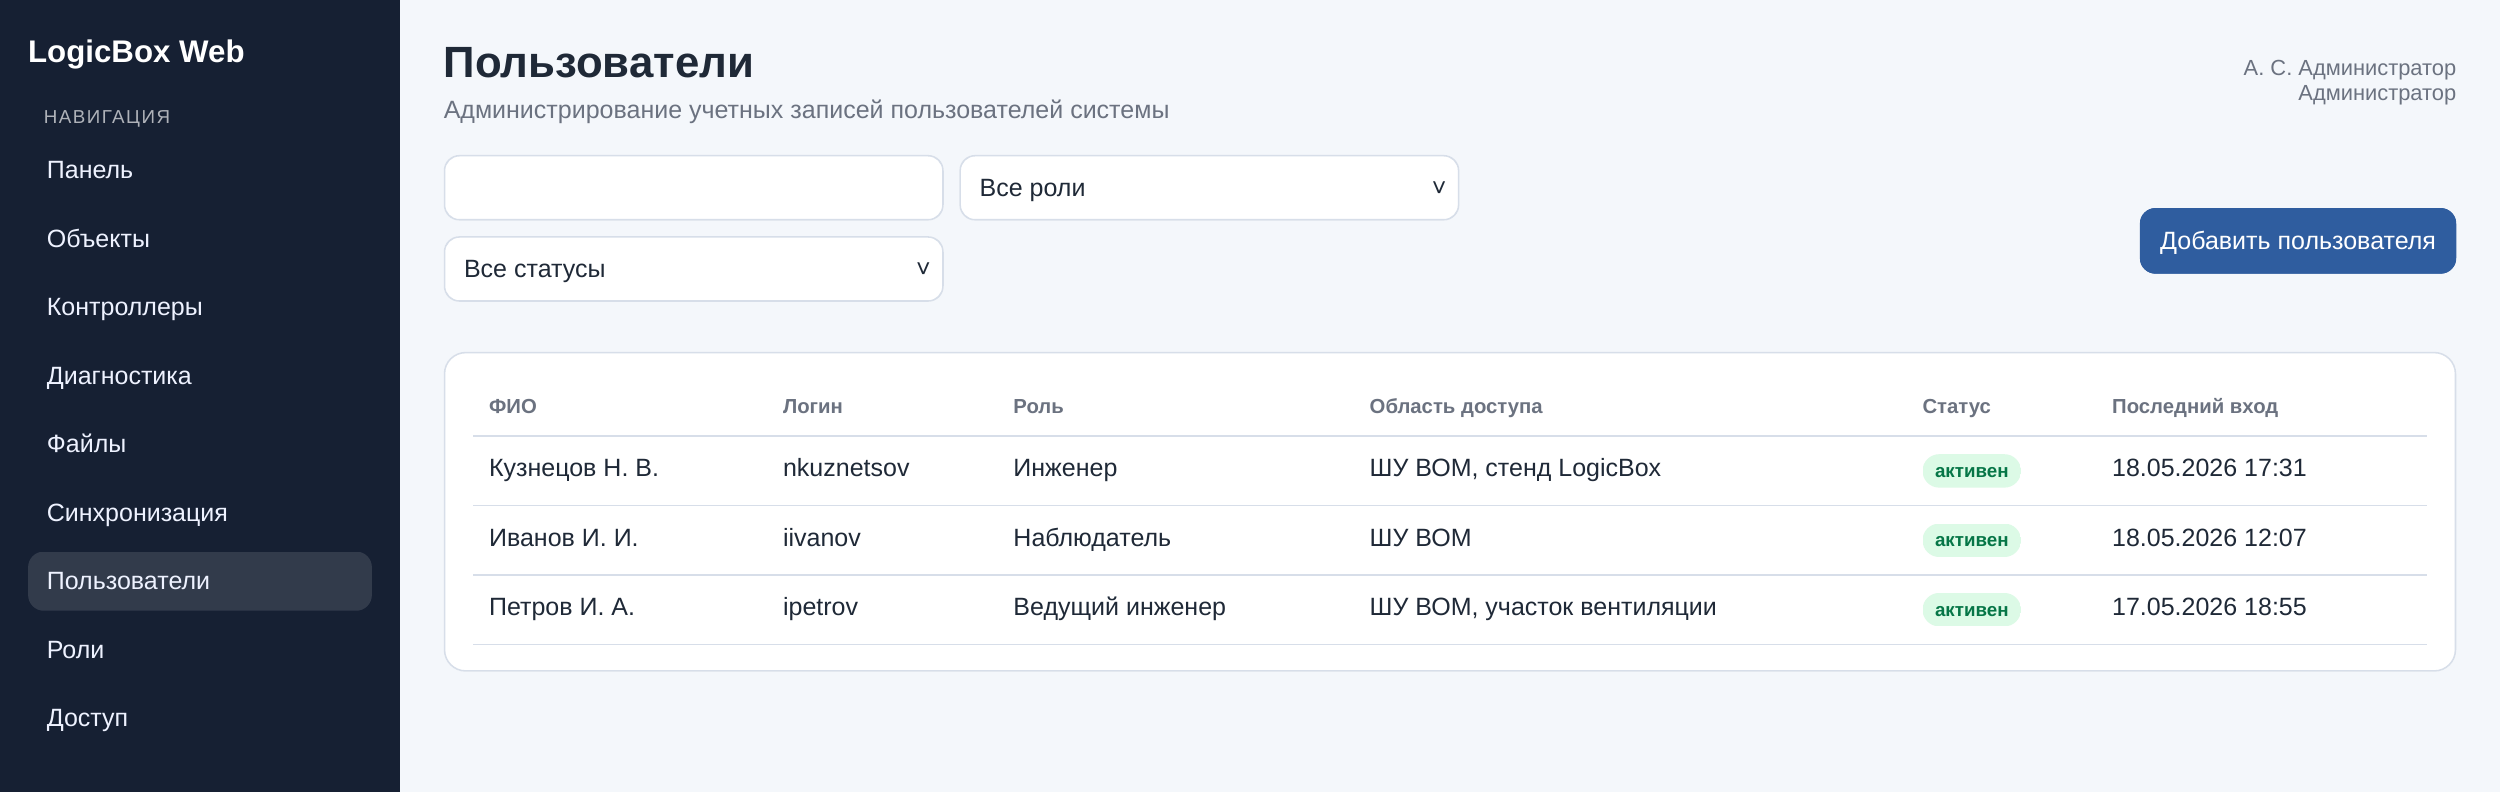
\includegraphics[width=0.90\textwidth,height=0.22\textheight,keepaspectratio]{images/mockups/admin_users.png}
    \caption{Администрирование пользователей}
\end{figure}
\vspace{2pt}

\begin{figure}[H]
    \centering
    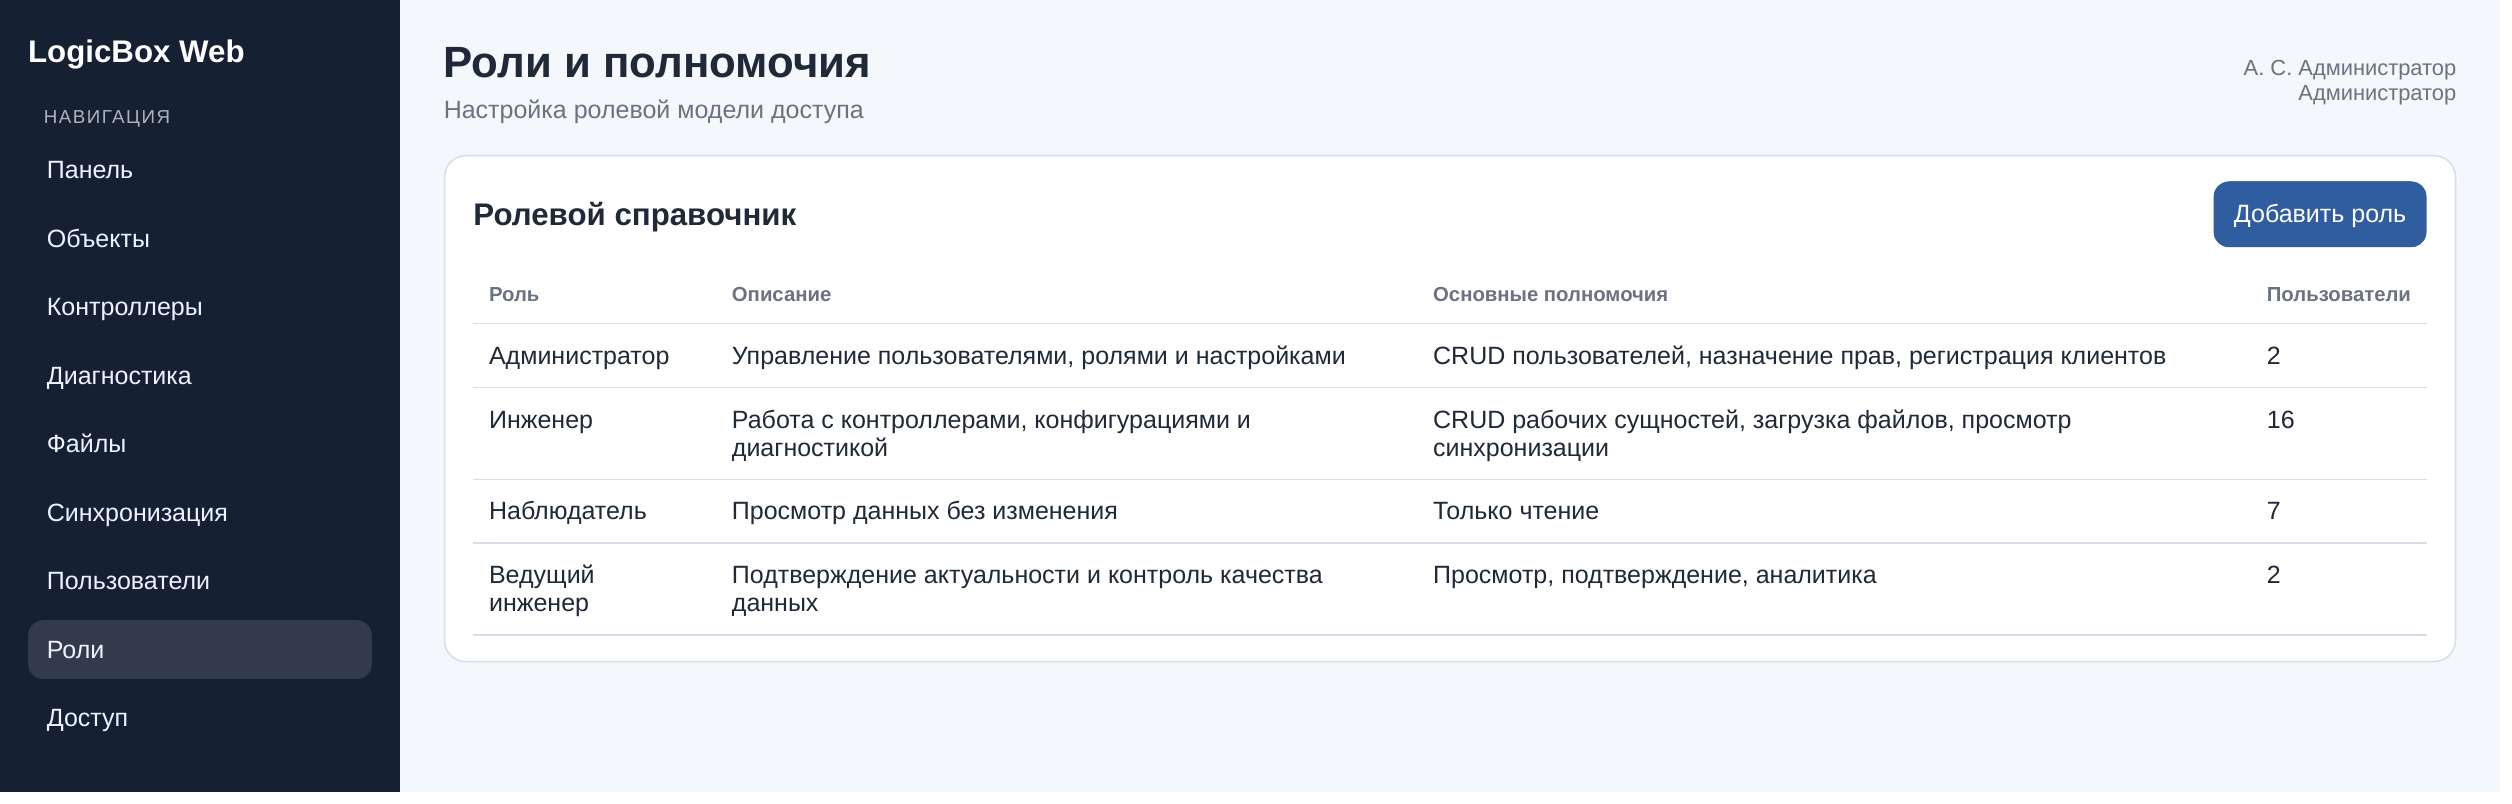
\includegraphics[width=0.90\textwidth,height=0.22\textheight,keepaspectratio]{images/mockups/admin_roles.png}
    \caption{Администрирование ролей}
\end{figure}
\vspace{2pt}

\begin{figure}[H]
    \centering
    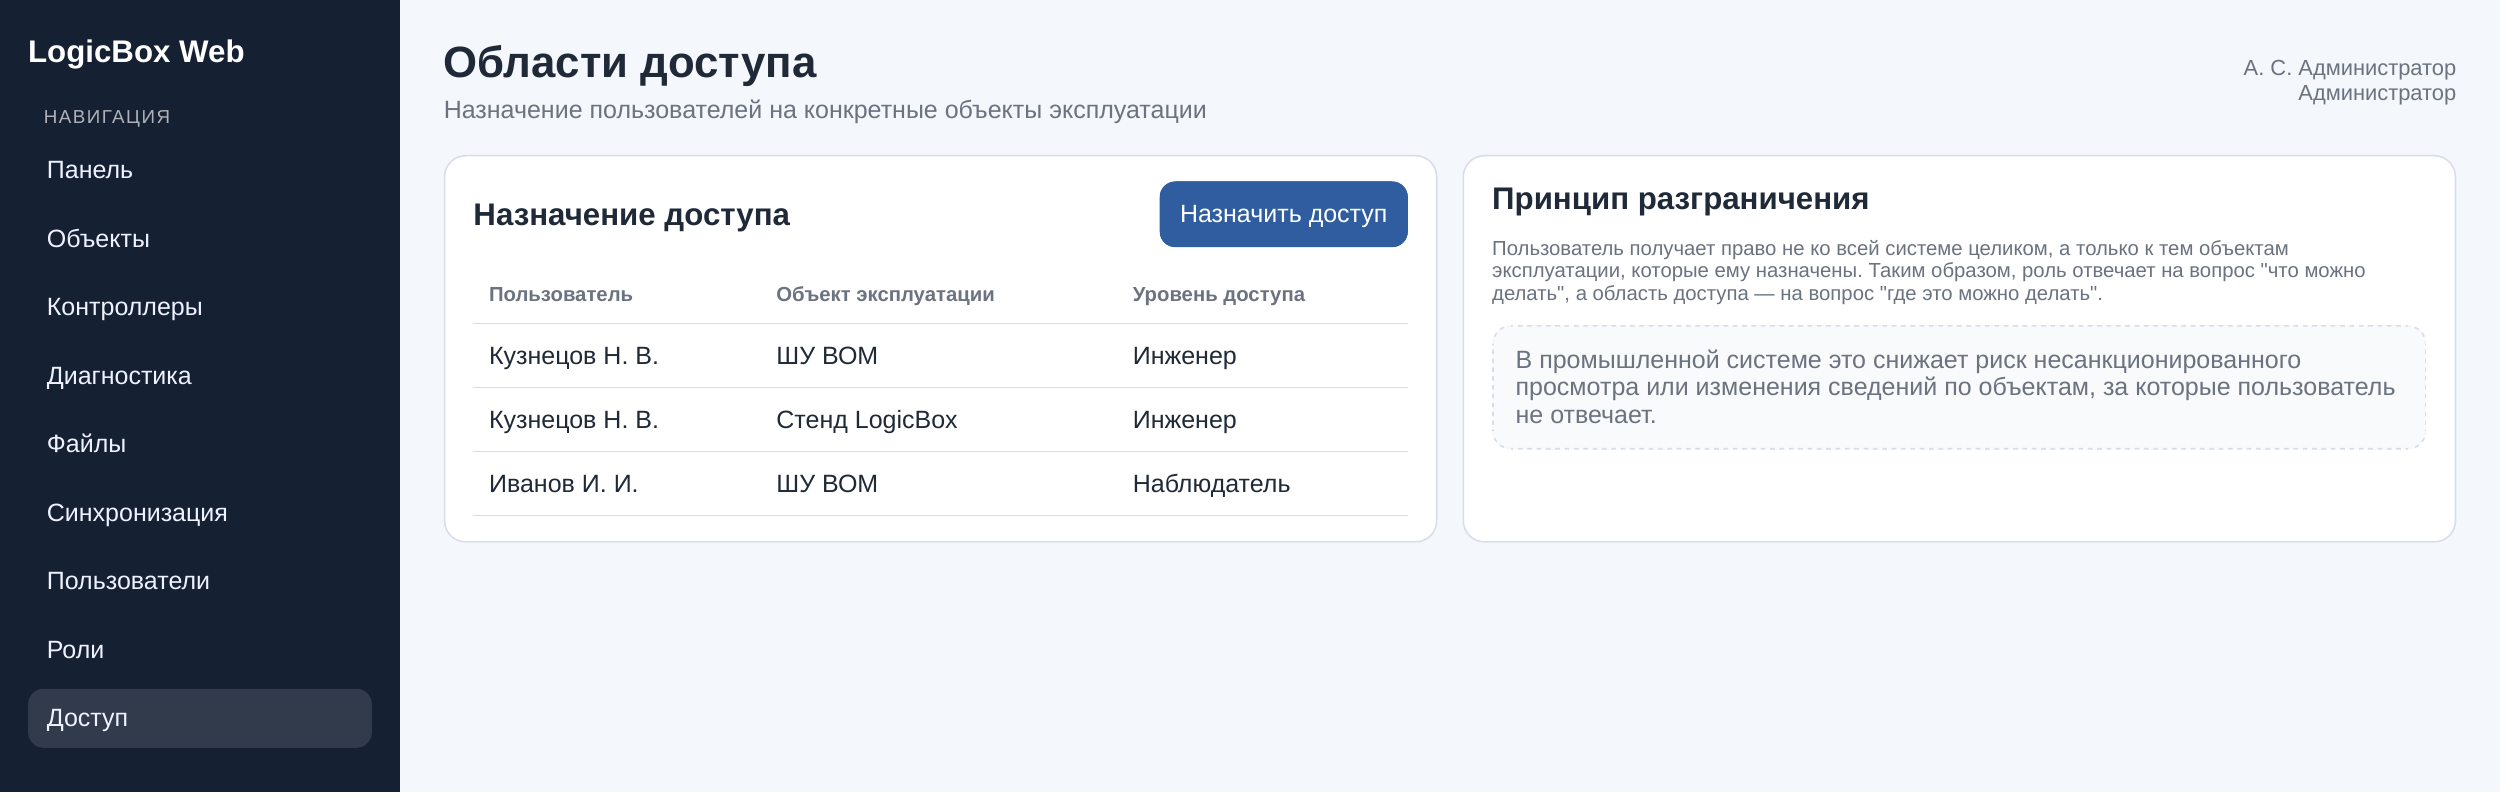
\includegraphics[width=0.90\textwidth,height=0.22\textheight,keepaspectratio]{images/mockups/admin_access.png}
    \caption{Назначение областей доступа}
\end{figure}
\vspace{2pt}

\begin{figure}[H]
    \centering
    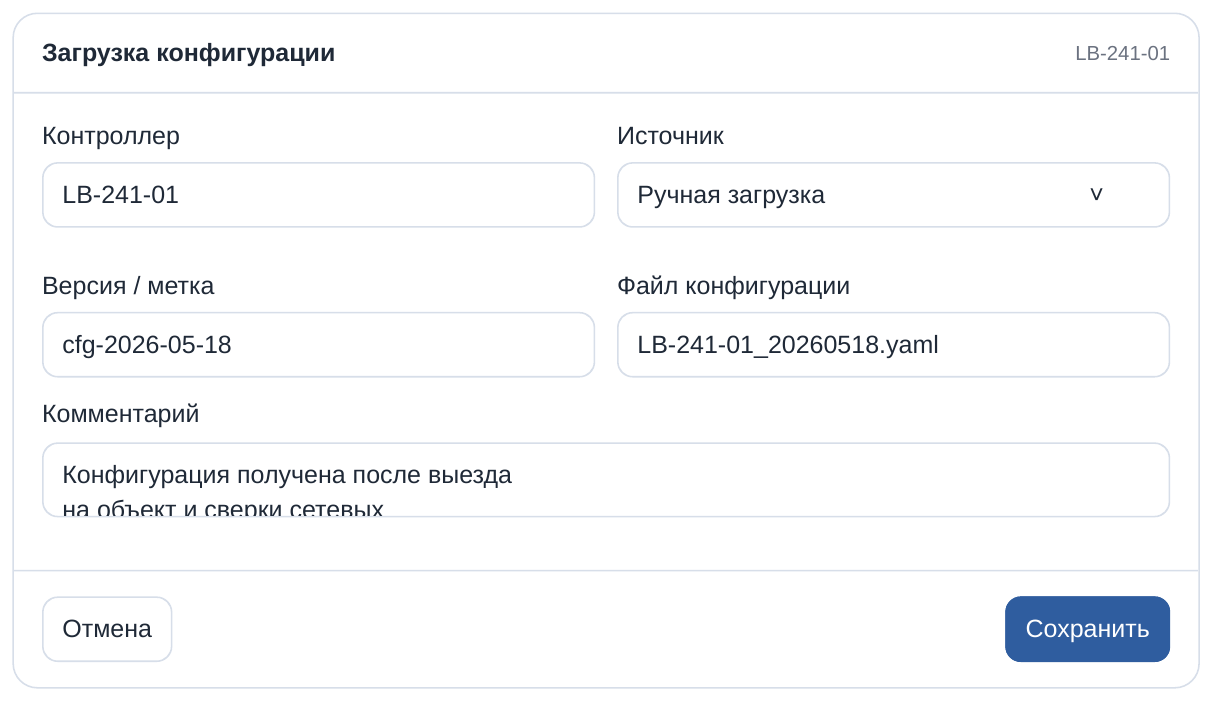
\includegraphics[width=0.90\textwidth,height=0.18\textheight,keepaspectratio]{images/mockups/modal_config_upload.png}
    \caption{Модальное окно загрузки конфигурации}
\end{figure}
\vspace{2pt}

\begin{figure}[H]
    \centering
    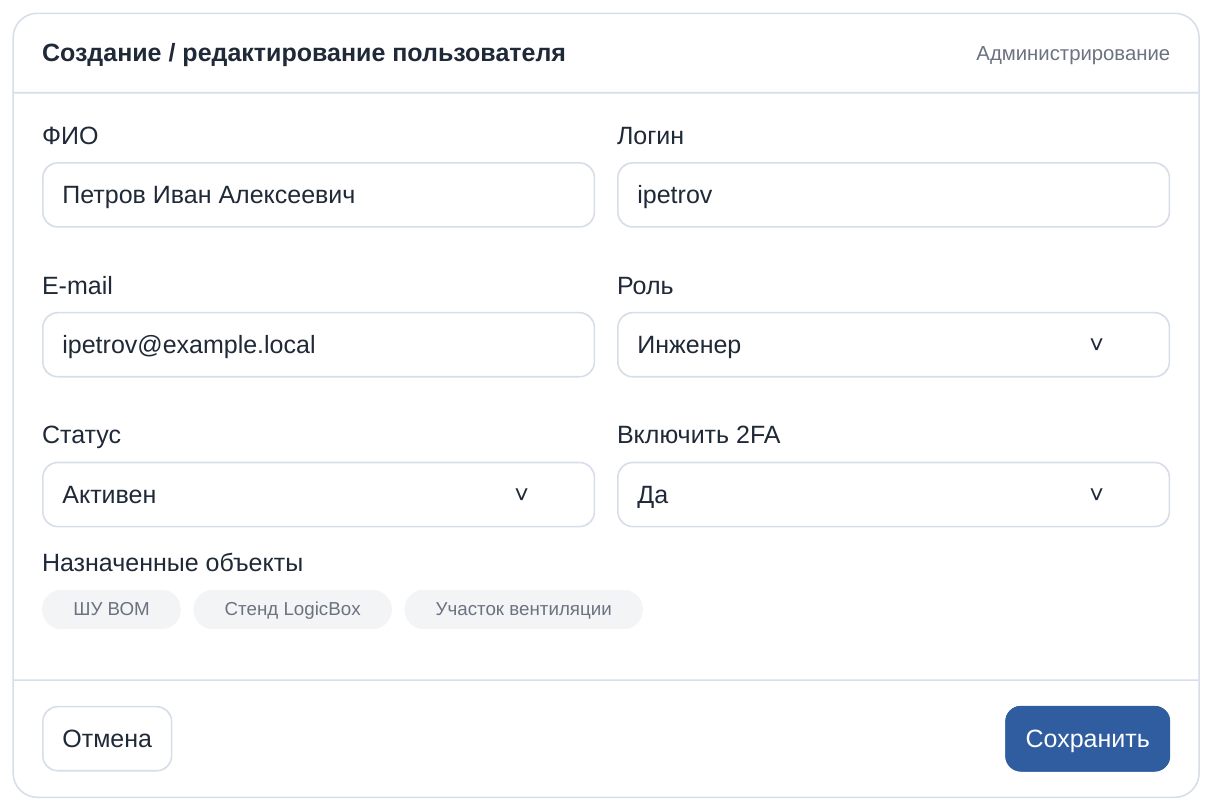
\includegraphics[width=0.90\textwidth,height=0.18\textheight,keepaspectratio]{images/mockups/modal_user_edit.png}
    \caption{Модальное окно создания или редактирования пользователя}
\end{figure}
\vspace{2pt}

\begin{figure}[H]
    \centering
    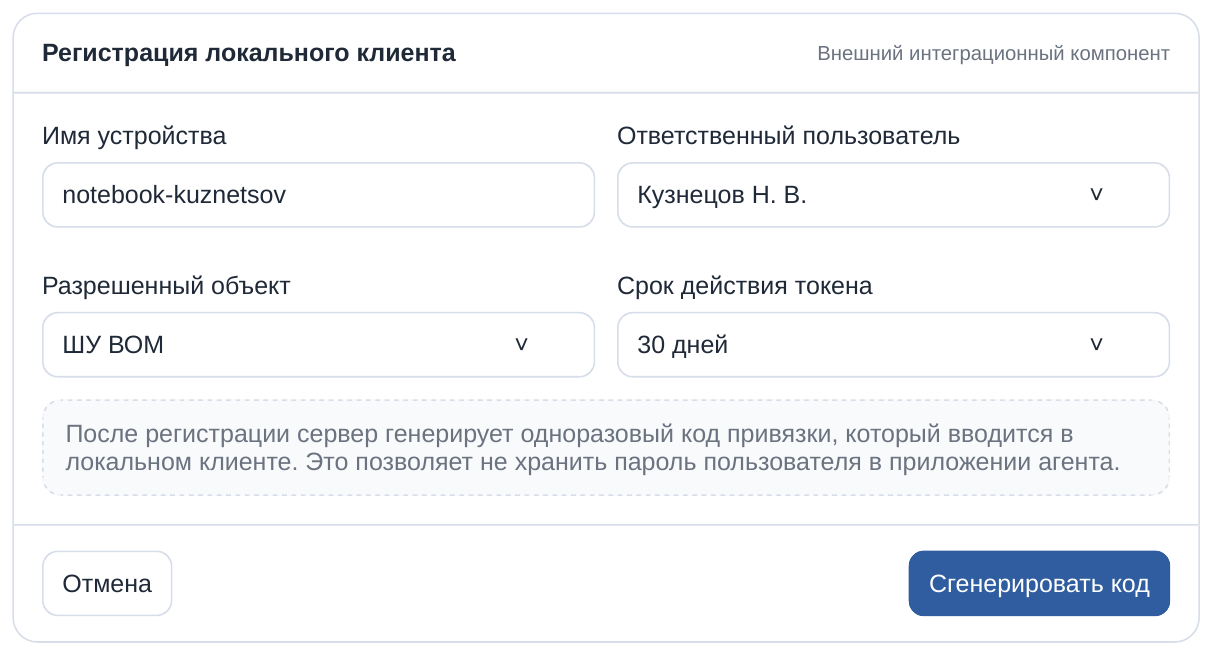
\includegraphics[width=0.90\textwidth,height=0.18\textheight,keepaspectratio]{images/mockups/modal_agent_registration.png}
    \caption{Модальное окно регистрации локального клиента}
\end{figure}
\vspace{2pt}

\begin{figure}[H]
    \centering
    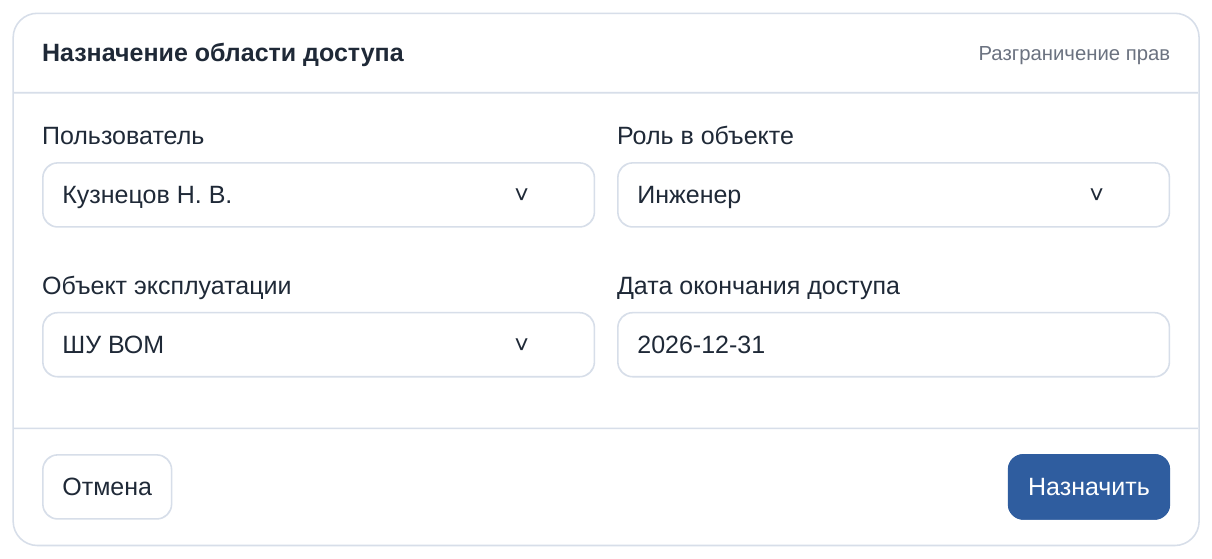
\includegraphics[width=0.90\textwidth,height=0.18\textheight,keepaspectratio]{images/mockups/modal_scope_assign.png}
    \caption{Модальное окно назначения области доступа}
\end{figure}
\vspace{2pt}

\begin{figure}[H]
    \centering
    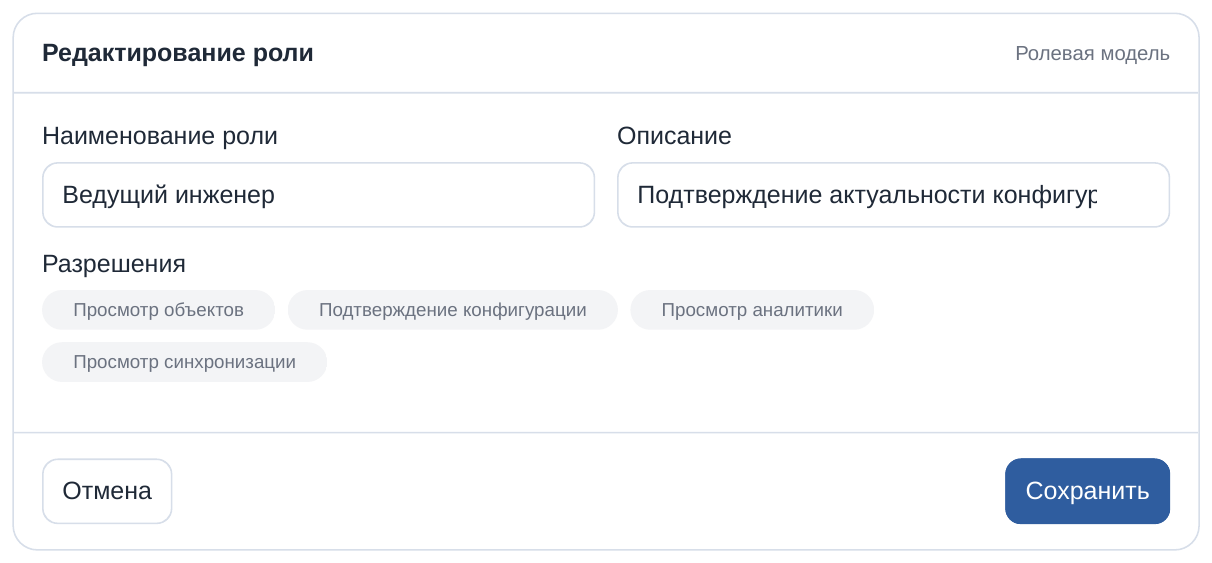
\includegraphics[width=0.90\textwidth,height=0.18\textheight,keepaspectratio]{images/mockups/modal_role_edit.png}
    \caption{Модальное окно редактирования роли}
\end{figure}
\vspace{2pt}

\begin{figure}[H]
    \centering
    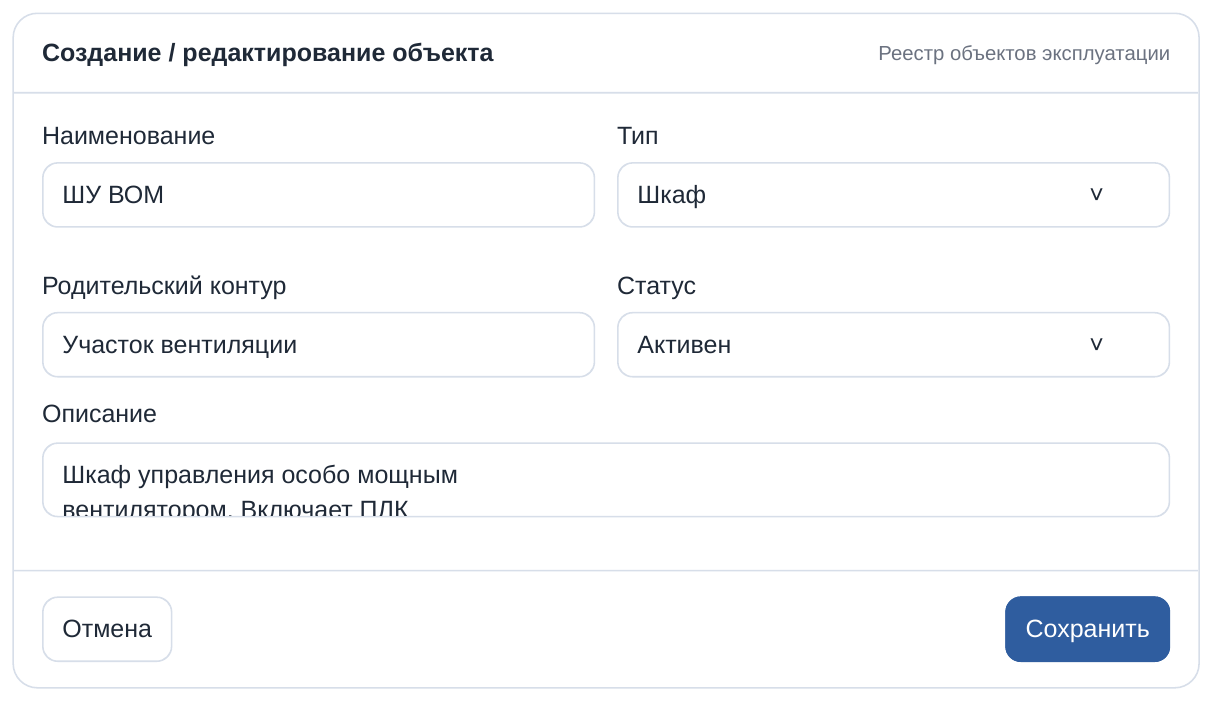
\includegraphics[width=0.90\textwidth,height=0.18\textheight,keepaspectratio]{images/mockups/modal_object_edit.png}
    \caption{Модальное окно редактирования объекта эксплуатации}
\end{figure}
\vspace{2pt}

\begin{figure}[H]
    \centering
    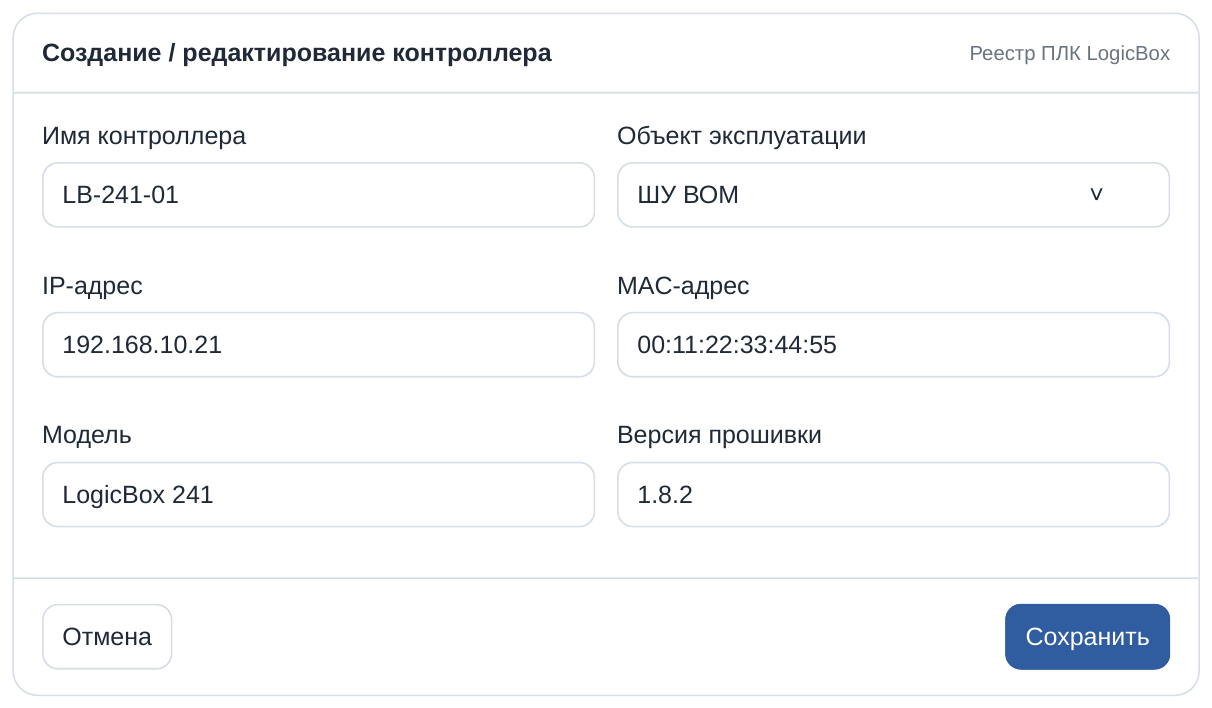
\includegraphics[width=0.90\textwidth,height=0.18\textheight,keepaspectratio]{images/mockups/modal_controller_create.png}
    \caption{Модальное окно создания или редактирования контроллера}
\end{figure}
\vspace{2pt}

\begin{figure}[H]
    \centering
    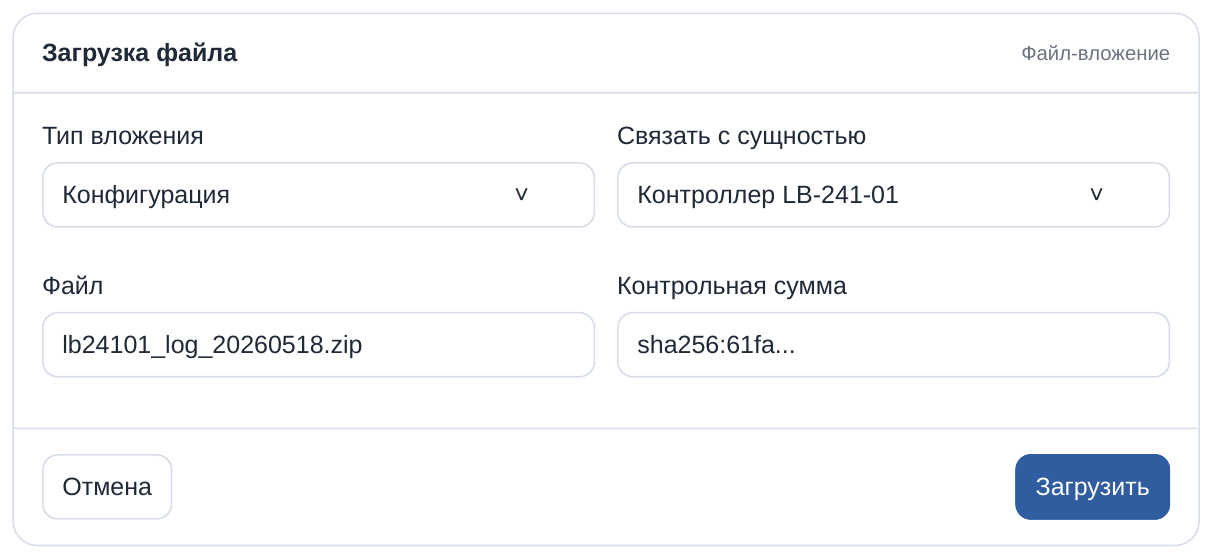
\includegraphics[width=0.90\textwidth,height=0.18\textheight,keepaspectratio]{images/mockups/modal_file_upload.png}
    \caption{Модальное окно загрузки файла-вложения}
\end{figure}
\vspace{2pt}

\begin{figure}[H]
    \centering
    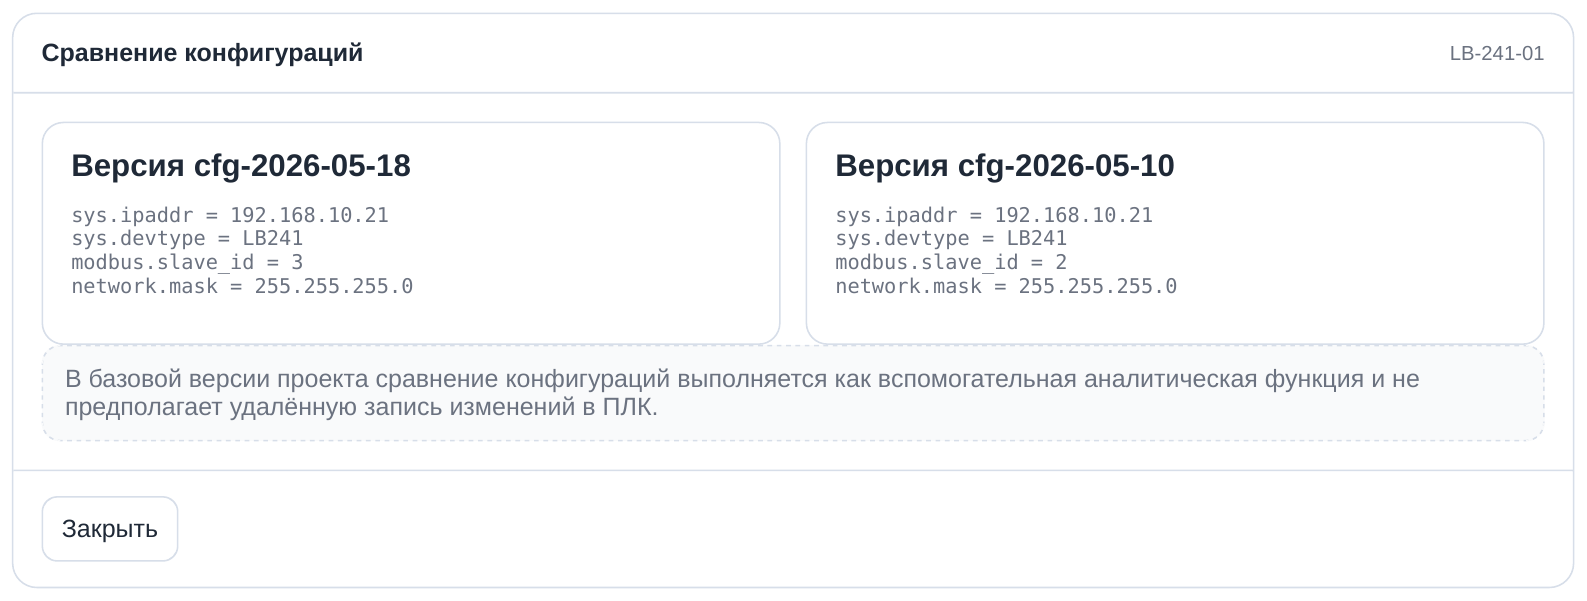
\includegraphics[width=0.90\textwidth,height=0.18\textheight,keepaspectratio]{images/mockups/modal_config_compare.png}
    \caption{Модальное окно сравнения конфигураций}
\end{figure}
\vspace{2pt}
